
\chapter{Hệ điều hành}
\label{chap:4}

\minitoc
\vspace{0.5cm}
\noindent
Trong chương này, ta sẽ xem xét về Hệ Điều Hành, là tập các gói phần mềm để điều phối các
 hoạt động bên trong của máy cũng như để giao tiếp với thế giới bên ngoài. Cũng chính điều
hành của máy đã chuyển đổi phần cứng thành các công cụ có ích. Ta sẽ cùng tìm hiểu xem hệ
điều hành làm những gì và làm như thế nào.

\textbf{Hệ điều hành} là phần mềm điều khiển toàn bộ thao tác của máy tính. Nó cung cấp
cho người dùng cách lưu trữ và tìm kiếm các tập tin, giao diện để người dùng yêu cầu thực
hiện chương trình, và môi trường cần thiết để thực hiện các chương trình được yêu cầu.


Hệ điều hành được nhiều người biết đến nhất có lẽ là Windows, nó có nhiều phiên bản khác
nhau và được viết bởi hãng Microsoft. Một ví dụ khác là UNIX, thường được dùng cho các hệ
thống máy tính lớn cũng như cho các máy PC. Trên thực tế, Mac OS, hệ điều hành của Apple
chuyên cho dòng máy Mac, được viết dựa trên nhân của UNIX. Một ví dụ khác nữa là
GNU/Linux, dùng cho cả hệ thống lớn và nhỏ, nó gốc được phát triển bởi cộng đồng những
người say mê và không vì mục đích thương mại.  Hiện nay nó cũng được hỗ trợ bởi các công
ty lớn như IBM.

\begin{figure}
\begin{quotation}
\noindent
\textbf{Linux} \vspace{0.3cm}
\\
Nếu bạn đam mê máy tính và muốn thử nghiệm với các thành phần bên trong của một hệ điều
hành, vậy thì Linux là dành cho bạn. Linux là một hệ điều hành được thiết kế đầu tiên bởi
Linus~Torvald khi anh là sinh viên tại Trường Đại học Helsinki. Đây không phải là một sản
phẩm thuộc quyền sở hữu của ai cả và luôn có sẵn, cùng với mã nguồn và tài liệu, cũng
không có ai chịu trách nhiệm. Bởi vì nó luôn có sẵn ở dạng mã nguồn, nên nó đã trở nên phổ
biến trong giới những người say mê máy tính, các sinh viên học hệ điều hành, và những
người lập trình. Hơn nữa, Linux được thừa nhận là một trong những hệ điều hành mềm dẻo
nhất sẵn có ngày nay. Vì lý do này, nhiều công ty hiện nay đã đóng gói và đưa ra thị
trường nhiều phiên bản Linux ở dạng dễ sử dụng, và các sản phẩm này hiện nay đang cạnh
tranh với các hệ điều hành thương mại khác đã có mặt từ lâu trên thị trường. Bạn có thể
tham khảo thêm thông tin về Linux tại trang web \url{http://www.linux.org}.
\end{quotation}
\end{figure}
 

\section{Lịch sử  các hệ điều hành}
\label{sec:31}

Máy tính trong những năm $1940$ và $1950$ rất không mềm dẻo và hiệu quả. Chúng chiếm hết
cả căn phòng, và việc thực hiện chương trình yêu cầu chuẩn bị nhiều thứ: lắp các băng từ,
đặt các bìa đục lỗ vào ổ đọc, bố trí các chuyển mạch,... Việc thực hiện chương trình (ở
đây ta gọi là \textbf{công việc} (job)) được xử lý như một hoạt động riêng biệt, và máy đã
phải đã được chuẩn bị sẵn sàng từ trước để thực hiện chương trình này.  Khi chương trình
thực hiện xong, nếu ta muốn thực hiện tiếp chương trình khác thì ta lại phải lưu trữ trước
mọi băng, thẻ đục lỗ,... Khi có nhiều người muốn chia sẻ một máy, họ phải đăng ký trước
thời gian dùng máy. Trong khoảng thời gian được cấp phép, máy hoàn toàn thuộc quyền điều
khiển của người dùng. Phiên làm việc bao gồm cài đặt chương trình (mất rất nhiều thời
gian) và chạy chương trình (trong khoảng thời gian rất ngắn). Mọi thứ luôn phải làm vội
vàng vì luôn có người đang kiên nhẫn chờ để dành máy.

Trong môi trường như vậy, các hệ điều hành ban đầu chỉ nhằm đơn giản hoá việc cài đặt
chương trình và hợp lý hoá việc chuyển đổi giữa các công việc. Những cải tiến đầu tiên là
tách riêng người sử dụng và thiết bị nhằm tránh việc có quá nhiều người ra vào phòng máy
tính. Với mục đích này, các phòng máy luôn có người trực máy. Khi người dùng muốn thực
hiện một chương trình, anh ta phải gửi chương trình, dữ liệu cần chạy, và các chỉ dẫn cụ
thể về chương trình cho người trực máy, và đợi để nhận lại kết quả chạy. Về phía người
trực máy, anh ta phải bật máy, đưa các thông tin này vào thiết bị lưu trữ khối của máy nơi
một chương trình được gọi là hệ điều hành có thể đọc và thực hiện chúng. Đây là bắt đầu
của \textbf{xử lý theo lô}--các công việc cần thực hiện được tập hợp lại và thực hiện mà
không cần tương tác với người sử dụng.


Trong các hệ thống xử lý theo lô, các công việc đợi thực hiện nằm trong một thiết bị lưu
trữ khối. Thiết bị này được gọi là \textbf{hàng đợi công việc} (job queue) (Hình
\ref{fig:fig3.1}). Một \textbf{hàng đợi} là một tập các đối tượng (trong trường hợp này là
các công việc) được tổ chức theo kiểu \textbf{vào trước, ra trước} (gọi tắt là FIFO). Có
nghĩa rằng, các đối tượng được lấy ra khỏi hàng đợi theo thứ tự chúng được đưa vào. Trên
thực tế, hầu hết các hàng đợi không tổ chức chặt chẽ theo cấu trúc FIFO mà xem xét theo độ
ưu tiên của từng đối tượng. Các hệ điều hành nói chung đều cho phép xem xét các công việc
theo độ ưu tiên. Bởi vậy, một công việc nằm trong hàng đợi dù sắp đến lượt vẫn có thể bị
đẩy về sau bởi một công việc khác có độ ưu tiên cao hơn.

\begin{figure}[bt]
\centering
    \scalebox{0.35}{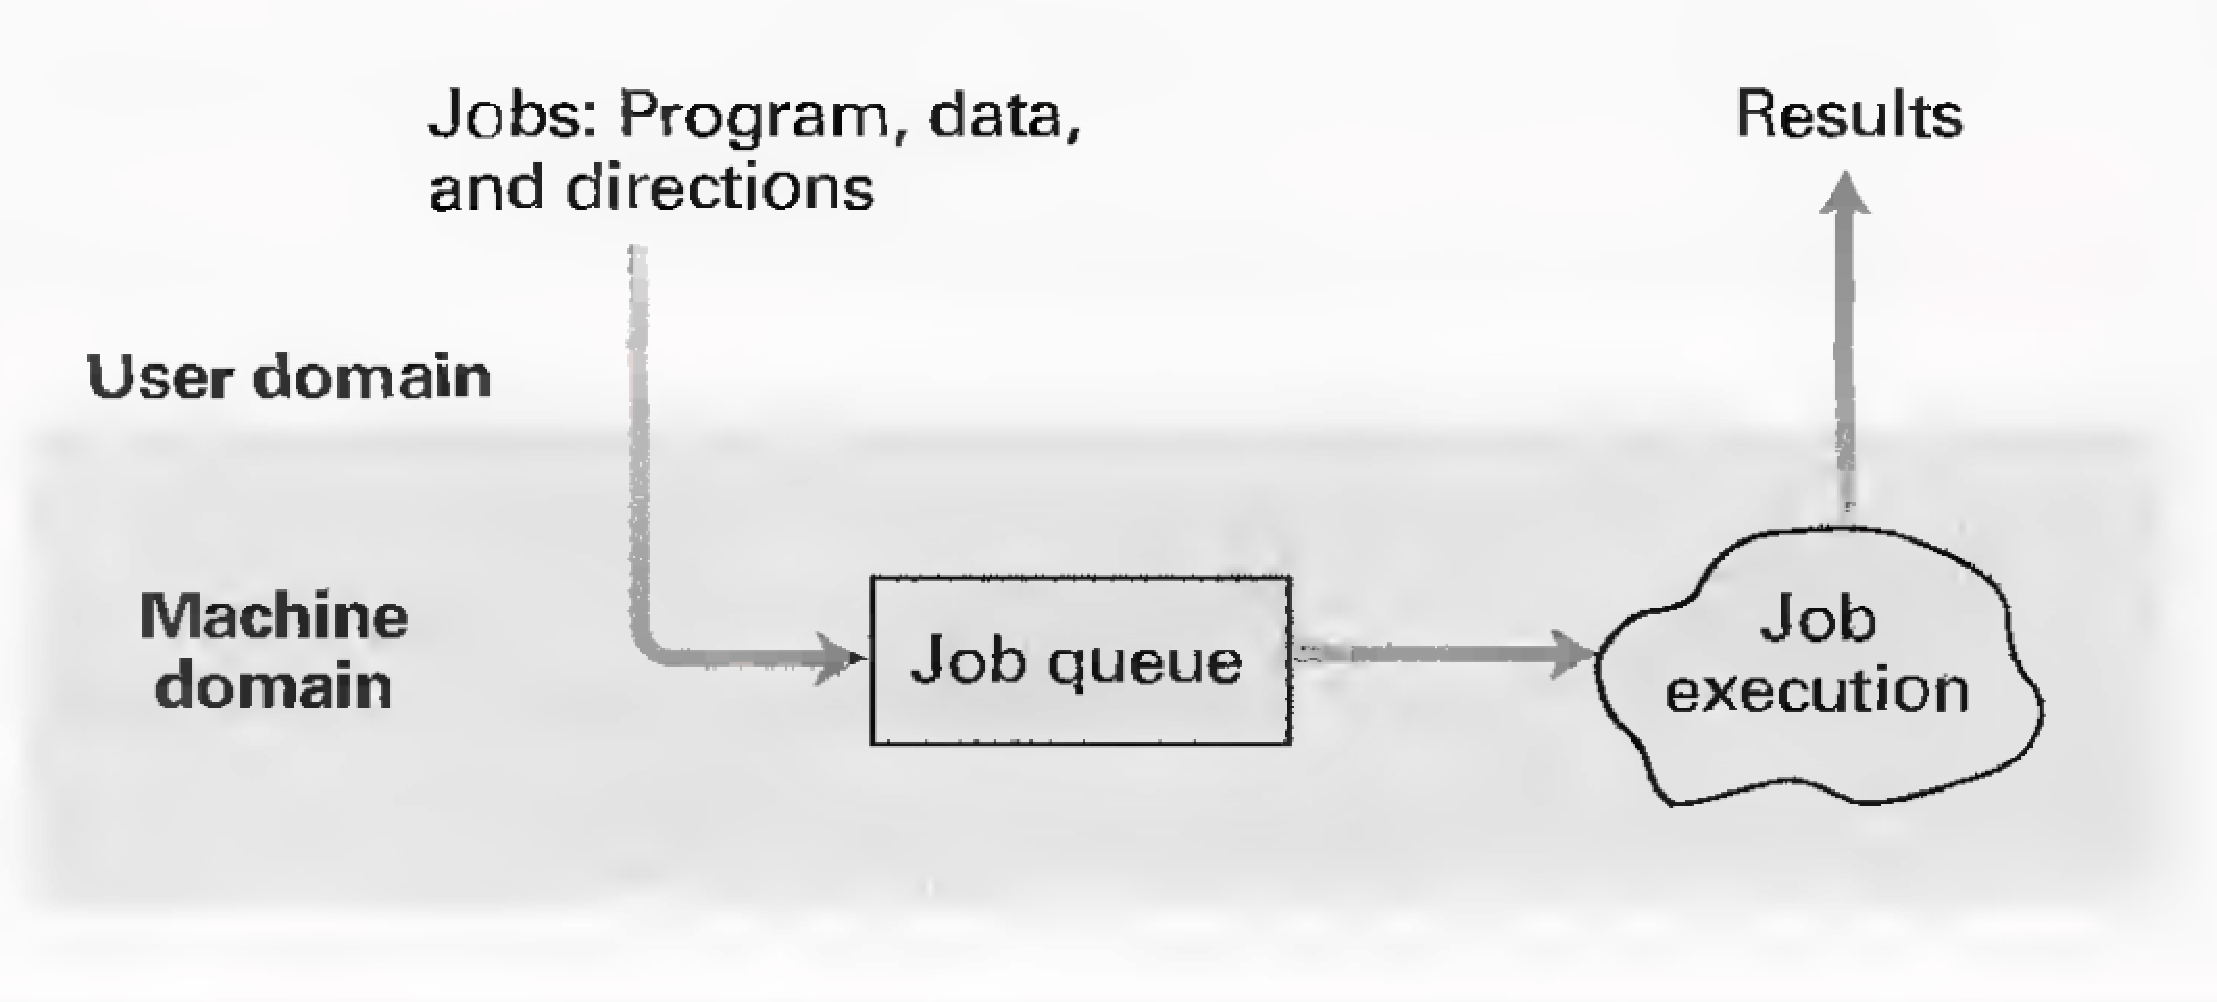
\includegraphics{ch4/fig31.pdf}}
\caption{Xử lý theo lô}
  \label{fig:fig3.1}
\end{figure}

Trong các hệ thống xử lý theo lô trước đây, mỗi công việc đi kèm với bởi một tập các chỉ
thị giải thích các bước yêu cầu người trực máy chuẩn bị theo đặc thù của công việc đó. Các
chỉ thị này được mã hoá, dùng một hệ thống gọi là ngôn ngữ điều khiển công việc (JCL). Tập
chỉ thị này được lưu trữ cùng với công việc trong hàng đợi công việc. Khi một công việc
được chọn để thực hiện, hệ điều hành in các chỉ thị này ra máy in để người trực máy tính
có thể đọc và làm theo. Ngày nay, ta vẫn thấy cách giao tiếp này, ví dụ như các báo lỗi
của hệ điều hành: ``no dial tone'', ``ổ đĩa không truy cập được'' hay ``máy in không trả
lời''.

Một trở ngại trong việc sử dụng người trực máy làm trung gian là người dùng phải gửi công
việc cho người trực máy, và do đó họ không thể tương tác được với công việc của họ. Cách
tiếp cận này có thể phù hợp với một số kiểu ứng dụng, ví dụ như xử lý bảng lương ở đó tất
cả mọi dữ liệu và cách xử lý đã được xác định trước. Tuy nhiên, trong nhiều trường hợp
cách này là không chấp nhận được, ví dụ như trong hệ thống đặt vé ở đó việc đặt và huỷ vé
phải được báo cáo ngay khi chúng xuất hiện, trong hệ thống xử lý văn bản ở đó tài liệu
được viết và viết lại liên tục, hay trong các trò chơi máy tính ở đó người dùng luôn phải
tương tác với máy.

Để thích nghi với các nhu cầu này, người ta đã phát triển các hệ điều hành mới cho phép
các chương trình thực hiện giao tiếp với người sử dụng qua trạm cuối ở xa--đặc điểm này
được gọi là \textbf{xử lý tương tác} (Hình \ref{fig:fig3.2}). Vào thời kỳ đó, các thiết bị
đầu cuối (cũng được gọi là máy trạm) chỉ có tính năng giống máy chữ--người dùng nhập dữ
liệu và đọc câu trả lời đã được máy tính in trên giấy.

\begin{figure}[tb]
  \centering \scalebox{0.35}{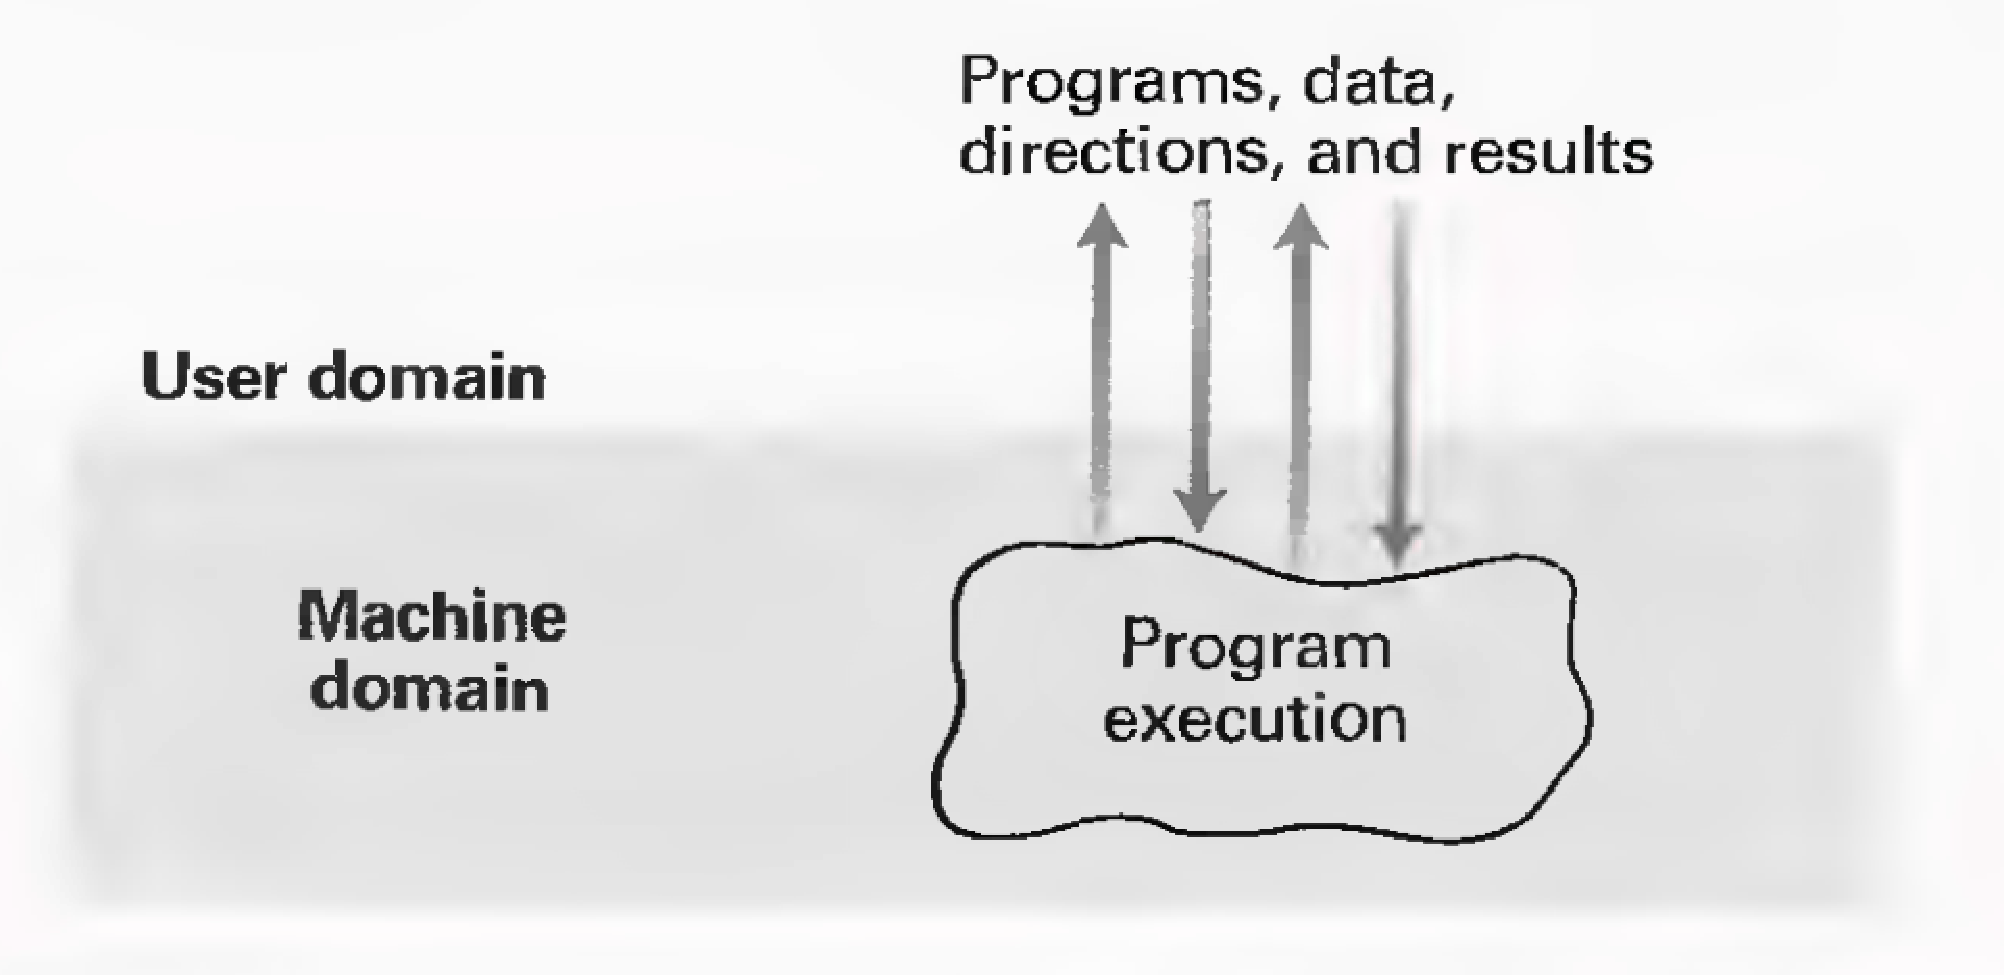
\includegraphics{ch4/fig32.pdf}}
\caption{Xử lý tương tác}
  \label{fig:fig3.2}
\end{figure}

Để việc xử lý tương tác thành công, điều hết sức quan trọng là các hoạt động của máy tính
phải đủ nhanh để phối hợp với các thao tác của người dùng thay vì ép người dùng phải chờ
đợi (ta có thể chờ đợi các các nhiệm vụ xử lý tiền lương thực hiện, nhưng không thể chấp
nhận nếu trong ứng dụng xử lý văn bản, máy tính không trả lời dấu nhắc lệnh khi các ký tự
được đánh). Các phục vụ của máy tính thoả mãn yêu cầu về thời gian được gọi là \textbf{xử
  lý thời gian thực}. Có nghĩa rằng, máy tính thực hiện nhiệm vụ đủ nhanh để để có thể
theo kịp các hoạt động của môi trường bên ngoài (thế giới thực).

Nếu hệ thống tương tác chỉ phục vụ một người dùng tại một thời điểm, vậy nó không gặp vấn
đề gì trong xử lý thời gian thực. Nhưng các máy tính trong những năm $1960$ và~$1970$ rất
đắt tiền, bởi vậy tại mỗi thời điểm, mỗi máy phải phục vụ rất nhiều người dùng. Họ làm
việc qua thiết bị đầu cuối ở xa để chuyển các phục vụ tương tác với máy, và vấn đề thời
gian thực trở thành một trở ngại. Nếu hệ điều hành cứ nhất định thực hiện một nhiệm vụ tại
một thời điểm, vậy thì chỉ một người dùng có thể thoả mãn phục vụ thời gian thực.

Một giải pháp cho vấn đề này là thiết kế hệ điều hành sao cho nó có thể chuyển việc thực
hiện các công việc khác nhau theo một chiến lược gọi là \textbf{chia sẻ thời gian thực},
đó là kỹ thuật chia thời gian thành các khoảng và sau đó hạn chế việc thực hiện mỗi công
việc trong một khoảng thời gian nhất định tại một thời điểm. Khi kết thúc mỗi khoảng, công
việc hiện hành bị đặt tạm ra bên ngoài và cho phép công việc khác tiếp tục thực hiện trong
khoảng tiếp theo. Bằng cách tráo đổi các công việc trước và sau một cách nhanh chóng theo
cách này, nó tạo ra cảm giác có nhiều công việc được chạy đồng thời. Phụ thuộc vào kiểu
công việc đang thực hiện, các hệ thống chia sẻ thời gian thực trước đây đã có thể cho phép
xử lý thời gian thực chấp nhận được với khoảng $30$ người sử dụng đồng thời. Ngày nay,
chia sẻ thời gian thực được sử dụng với hệ thống đơn người dùng cũng tốt như đa người
dùng, mặc dù về hình thức nó được gọi là \textbf{đa nhiệm}, để chỉ các hệ thống cho phép
(về mặt cảm giác) tại một thời điểm có thể có nhiều nhiệm vụ được thực hiện đồng thời.

Với sự phát triển của hệ điều hành đa người dùng và chia sẻ thời gian thực, một máy tính
đã được cấu hình như máy trung tâm kết nối với nhiều máy trạm. Từ các máy trạm này, người
dùng có thể giao tiếp trực tiếp với máy tính bên ngoài phòng máy thay vì phải gửi yêu cầu
tới người trực máy. Các chương trình sử dụng chung được lưu trữ trước trong thiết bị lưu
trữ khối của máy và hệ điều hành đã được thiết kế để thực hiện các chương trình này theo
yêu cầu từ các máy trạm. Vai trò người trực máy dần bị phai nhoà.

Ngày nay, về cơ bản không còn người trực máy nữa, đặc biệt trong lĩnh vực máy tính cá nhân
ở đó người sử dụng chịu mọi trách nhiệm thay người trực máy. Thậm chí hầu hết các máy tính
lớn không còn cần có người quản lý. Giờ đây công việc của người trực máy đã được thay bằng
người quản trị hệ thống, người chịu trách nhiệm quản lý hệ thống máy tính--có nhiệm vụ
theo dõi và thực hiện cài đặt thiết bị mới và phần mềm, bắt người dùng tôn trọng các quy
định như tạo tài khoản mới và thiết lập giới hạn không gian lưu trữ khối cho nhiều người
dùng, và cố gắng điều phối để giải quyết vấn đề gây ra trong hệ thống--hơn là thao tác với
máy trực tiếp bằng tay.

Tóm là, hệ điều hành đã phát triển từ một chương trình chỉ thực hiện nhiệm vụ đơn giản là
lưu trữ và thực hiện chương trình thành một hệ thống phức tạp điều phối việc chia sẻ thời
gian, bảo trì chương trình và các file dữ liệu trong các thiết bị lưu trữ khối của máy, và
trả lời trực tiếp yêu cầu từ người dùng.
 
Nhưng sự phát triển của các hệ điều hành vẫn chưa dừng ở đó. Sự phát triển của máy đa bộ
xử lý đã dẫn tới các hệ điều hành thực hiện đa nhiệm bằng cách gán các nhiệm vụ khác nhau
cho các bộ xử lý khác nhau thay vì chia sẻ thời gian của một bộ xử lý. Các hệ điều hành
này phải vật lộn với các vấn đề như \textbf{cân bằng tải} (các nhiệm vụ được gán một cách
động tới các bộ xử lý khác nhau sao cho mọi bộ xử lý được sử dụng một cách hiệu quả) cũng
như \textbf{scaling} (chia các nhiệm vụ thành các nhiệm vụ con tương thích với số bộ xử lý
có sẵn). Hơn nữa, sự phát triển của các mạng máy tính với nhiều máy ở khoảng cách xa được
kết nối với nhau đã dẫn tới tính cần thiết của phần mềm hệ thống để điều phối các hoạt
động của mạng. Bởi vậy lĩnh vực mạng (ta sẽ nghiên cứu chi tiết ở Chương \ref{} ) là một
trong nhiều chủ đề mở rộng của các hệ điều hành--mục đích là phát triển một hệ điều hành
đơn cho mạng rộng thay vì một mạng gồm nhiều hệ điều hành riêng lẻ.

\subsection*{Câu hỏi \& Bài tập}
\begin{enumerate}
\item Cho các ví dụ về hàng đợi. Trong mỗi trường hợp, chỉ ra tình
  huống vi phạm với cấu trúc FIFO.

\item Các hoạt động nào dưới đây yêu cầu xử lý thời gian thực?
  \begin{enumerate}
  \item In các nhãn thư điện tử

  \item Chơi một trò chơi trên máy tính

  \item Hiện các ký tự ra màn hình như chúng được nhập vào từ bàn phím

  \item Thực hiện chương trình dự báo tình trạng nền kinh tế trong năm
    tới
  \end{enumerate}

\item Nêu sự khác nhau giữa hệ điều hành xử lý thời gian thực và hệ
  điều hành tương tác?

\item Nêu sự khác nhau giữa hệ điều hành chia sẻ thời gian và đa nhiệm?
\end{enumerate}







%%% Local Variables: 
%%% mode: latex
%%% TeX-master: "../tindaicuong"
%%% End: 

\section{Kiến trúc hệ điều hành}

Để hiểu cấu tạo của một hệ điều hành, đầu tiên ta sẽ xem xét các phần mềm tìm thấy
bên trong một hệ thống máy tính. Sau đó ta sẽ trọng tâm trên bản thân hệ điều hành.

\subsection*{Tổng quan về phần mềm}

Ta sẽ tiến hành phân loại phần mềm để có cái nhìn tổng quan về phần mềm.  Lược đồ
phân loại phần mềm như vậy cũng giống như cách mà người ta phân múi giờ để mọi người đặt
đồng hồ chung chứ không có ý nghĩa phân biệt giữa sự xuất hiện của bình minh và hoàng
hôn. Hơn nữa, trong trường hợp phân loại phần mềm, tính động của phần mềm và thiếu định
nghĩa chính xác dẫn tới các thuật ngữ mâu thuẫn. Ví dụ, người sử dụng hệ điều hành Windows
của Microsoft sẽ tìm thấy nhóm phần mềm ``Accessories'' và ``Administrative Tool'' gồm
những phần mềm nằm trong cả phần ứng dụng và lớp công cụ. Cách phân loại dưới đây được
nhìn theo nghĩa kinh nghiệm về tính mở rộng và tính động của chủ đề hơn là một phát biểu
được chấp nhận rộng rãi trong thực tế.

Ta bắt đầu bằng cách chia phần mềm máy tính thành hai phạm trù rộng: \textbf{phần mềm ứng
  dụng} và \textbf{phần mềm hệ thống} (xem Hình~\ref{fig:fig3.3}). Phần mềm ứng dụng bao
gồm các chương trình nhằm thực hiện các nhiệm vụ đặc biệt. Một máy tính được dùng để bảo
quản việc kiểm kê hàng hoá tồn kho của một nhà sản xuất sẽ có các phần mềm ứng dụng khác
với một máy tính được dùng bởi một kỹ sư điện tử. Các ví dụ phần mềm ứng dụng bao gồm:
bảng tính, hệ quản trị cơ sở dữ liệu, hệ thống xuất bản desktop, hệ thống kế toán, phần
mềm phát triển chương trình, và các trò chơi.

\begin{figure}[tb]
  \centering \scalebox{0.4}{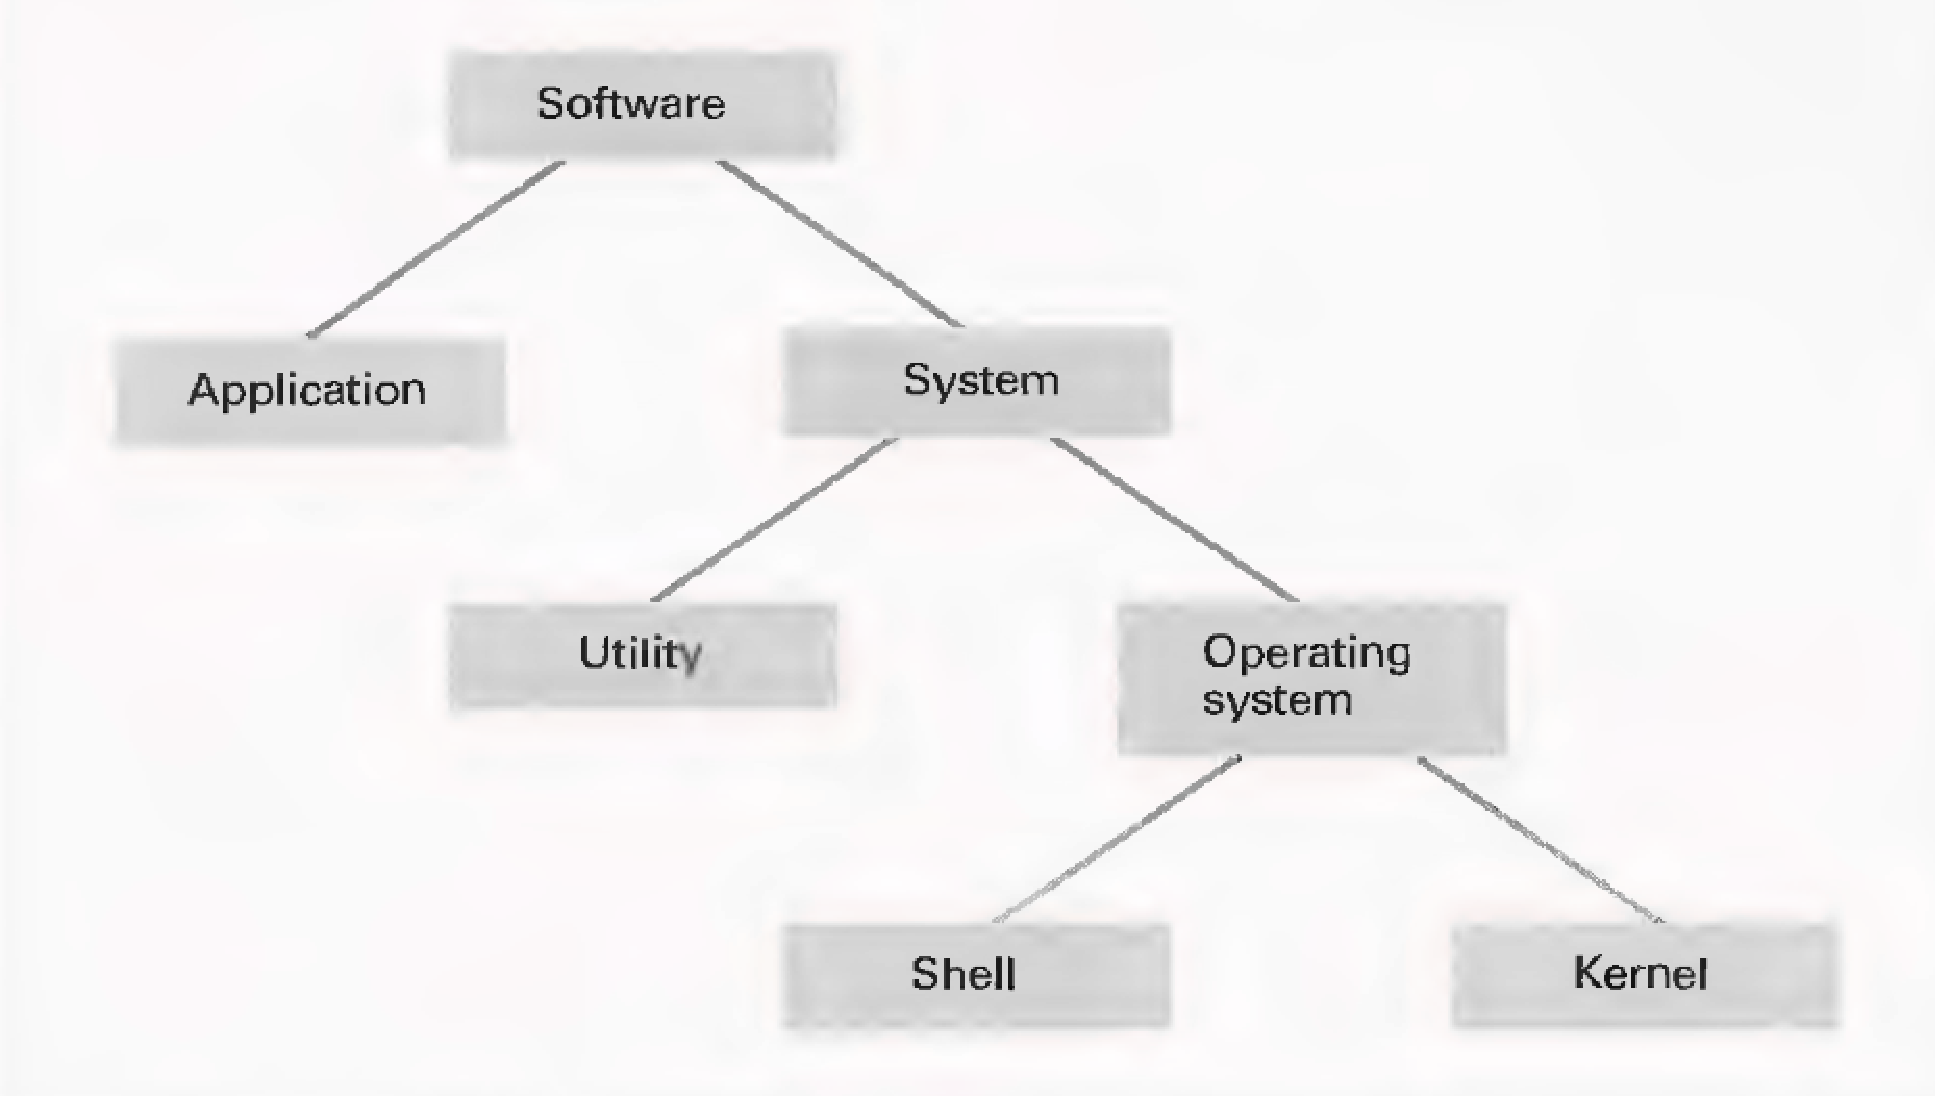
\includegraphics{ch4/fig33.pdf}}
  \caption{Phân loại phần mềm}
  \label{fig:fig3.3}
\end{figure}

Ngược lại với phần mềm ứng dụng là phần mềm hệ thống nhằm thực hiện các nhiệm vụ chung của
các hệ thống máy tính. Theo một nghĩa nào đó, phần mềm hệ thống cung cấp cơ sở hạ tầng cho
các phần mềm ứng dụng. Ta có thể ví nó với cơ sở hạ tầng của một quốc gia (chính
phủ, đường đi lại, các nghành phục vụ, viện tài chính,...) cung cấp cơ sở cho người dân
dựa vào sống theo cách của họ.

Bên trong các lớp các phần mềm hệ thống ta lại chia thành hai phạm trù: một là bản thân hệ
điều hành và hai là những phần mềm khác bao gồm các đơn vị phần mềm tập hợp lại dưới dạng
\textbf{phần mềm công cụ}. Phần lớn phần mềm công cụ cài đặt các chương trình nhằm thực
hiện các hoạt động cơ bản của máy tính nhưng không có sẵn trong hệ điều hành. Theo một
nghĩa nào đó, phần mềm công cụ bao gồm các đơn vị phần mềm giúp mở rộng (cũng có thể để
tuỳ biến) khả năng của hệ điều hành. Ví dụ, chức năng format một đĩa từ hoặc sao chép một
files từ đĩa từ vào đĩa CD thường không được cài đặt bởi hệ điều hành nhưng nó được cung
cấp bởi phần mềm công cụ. Những ví dụ khác của phần mềm công cụ là phần mềm nén và giải
nén dữ liệu, phần mềm để trình diễn đa phương tiện, và phần mềm để thực hiện truyền thông
trong mạng.

Sử dụng các phần mềm công cụ cho phép phần mềm hệ thống có thể tuỳ biến dễ dàng hơn so với
việc đặt chúng có sẵn ngay trong hệ điều hành. Thật vậy, thông thường các công ty hoặc cá
nhân phải thay đổi, hoặc thêm, các phần mềm công cụ vào hệ điều hành trong máy của họ.

Không may mắn, việc phân biệt giữa phần mềm ứng dụng và phần mềm công cụ là không rõ
ràng. Theo quan điểm của chúng tôi, sự khác biệt là gói phần mềm này có là một phần trong
cơ sở hạ tầng phần mềm của máy hay không. Bởi vậy một ứng dụng mới có thể thuộc nhánh công
cụ nếu nó trở thành một công cụ cơ bản. Khi vẫn còn là dự án nghiên cứu, phần mềm để
truyền thông trên Internet đã được xem là phần mềm ứng dụng; ngày nay phần mềm kiểu này là
cơ bản cho hầu hết việc sử dụng PC và bởi vậy nó được phân loại là phần mềm công cụ.



Sự phân biệt giữa phần mềm công cụ và hệ điều hành cũng không rõ ràng. Ví dụ, luật chống
độc quyền ở Mỹ và Châu Âu đã đặt ra câu hỏi liên quan đến phần mềm như trình duyệt web
Internet Explorer và Media Player là một thành phần của hệ điều hành của Microsoft hay chỉ
là phần mềm công cụ mà Microsoft đã cố tình cho vào hệ điều hành nhằm mục đích cạnh tranh.


\subsection*{Các thành phần của một hệ điều hành}

Ta sẽ chú tâm vào thành phần bên trong một hệ điều hành. Để có thể thực hiện các hoạt động
được yêu cầu bởi những người dùng, hệ điều hành phải có khả năng giao tiếp. Thành phần của
một hệ điều hành thực hiện việc giao tiếp này thường được gọi là \textbf{shell}. Các shell
hiện đại thực hiện nhiệm vụ này thường theo hướng \textbf{giao diện đồ hoạ với người dùng
  (GUI)} trong đó các đối tượng cần thao tác như các file và chương trình, được biểu diễn
bằng các biểu tượng trên màn hình. Các hệ thống này cho phép hiểu lệnh của người dùng
thông qua việc trỏ tới các biểu tượng này. Việc này thường được thực hiện nhờ một thiết bị
cầm tay được gọi là chuột. Các shell cũ hơn thường giao tiếp với người dùng qua thông điệp
dạng văn bản sử dụng bàn phím và màn hình.



Mặc dù shell của hệ điều hành đóng vai trò quan trọng trong việc thiết lập các chức năng
của máy, các shell này đơn thuần chỉ là giao diện giữa người dùng và nhân (trái tim) của
hệ điều hành (Hình \ref{fig:fig3.4}). Ta phân biệt giữa shell và phần bên trong của hệ
điều hành như thế này bởi vì một số hệ điều hành cho phép người dùng lựa chọn các shell
khác nhau để có một giao diện phù hợp với từng đối tượng người dùng cụ thể. Ví dụ, người
dùng hệ điều hành UNIX có thể lựa chọn một trong nhiều shell như Bourne shell, C shell, và
Korn shell. Hơn nữa, những phiên bản trước của hệ điều hành Microsoft Windows về mặt cơ
bản đã được xây dựng nhằm thay thế các shell dựa trên văn bản đang sử dụng (trên hệ điều
hành MS-DOS) bằng một shell kiểu giao diện đồ hoạ, tuy nhiên khung của nó vẫn là MS-DOS.

\begin{figure}[tb]
  \centering \scalebox{0.4}{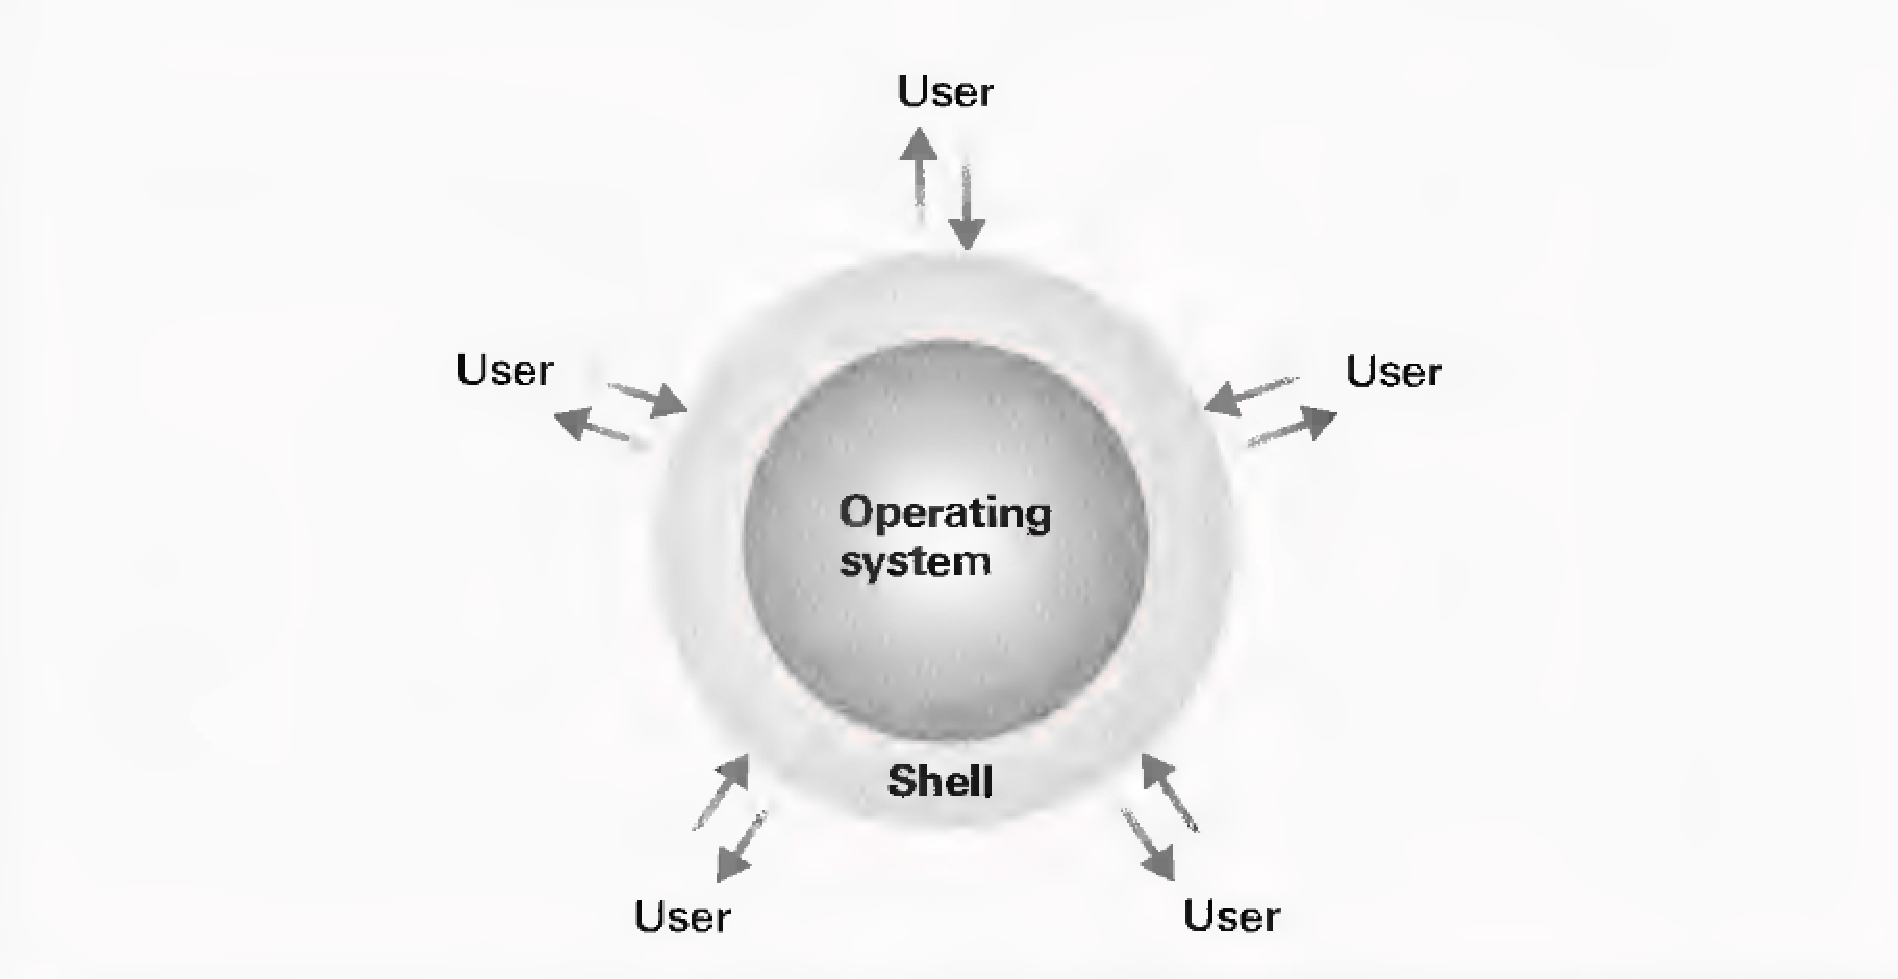
\includegraphics{ch4/fig34.pdf}}
  \caption{Shell như một giao diện giữa người dùng và hệ điều hành}
  \label{fig:fig3.4}
\end{figure}

Một thành phần quan trọng bên trong các shell đồ hoạ của ngày nay là \textbf{chương trình
  quản lý cửa sổ}, với các khối được cấp phát của không gian màn hình, được gọi là cửa sổ,
và mỗi các ứng dụng được gắn với mỗi cửa sổ. Khi một ứng dụng muốn hiện một thứ gì đó ra
màn hình, nó thông báo với trình quản lý cửa sổ, và trình quản lý cửa sổ sẽ đặt các hình
ảnh mong đợi vào trong cửa sổ gắn với ứng dụng. Từ đó, mỗi khi một nút chuột được nhấn,
chính trình quản lý cửa sổ sẽ tính toán vị trí của chuột trên màn hình và gọi ứng dựng
thích hợp tương ứng với thao tác của chuột.

Ngược lại với shell của hệ điều hành, phần bên trong của hệ điều hành được gọi là
\textbf{nhân} (kernel). Một nhân của hệ điều hành chứa các thành phần phần mềm thực hiện
các chức năng rất cơ bản yêu cầu bởi hệ thống máy tính. Một ví dụ là \textbf{trình quản lý
  file}, công việc của nó là phối hợp làm dễ dàng việc sử dụng thiết bị lưu trữ khối của
máy. Chính xác hơn, trình quản lý file chứa các bản ghi của mọi file nằm trong thiết bị
lưu trữ khối, gồm cả vị trí mỗi file được đặt, người dùng nào được phép truy cập vào file
nào, và bộ phận nào của lưu trữ khối sẵn sàng dành cho các file mới, hoặc mở rộng các file
đã tồn tại. Các bản ghi này được giữ ở một nơi lưu trữ trung gian chứa các file liên quan
sao cho mỗi thời điểm nơi trung gian được đặt trực tuyến, trình quản lý file có thể tìm
thấy chúng và biết có gì được lưu trữ ở phần trung gian này.

Để thích hợp với người dùng máy, hầu hết các trình quản lý file cho phép các file được
nhóm lại dưới dạng \textbf{thư mục} (directory hoặc folder). Cách tiếp cận này cho phép
người dùng tổ chức các file của anh hay chị ta theo mục đích bằng cách đặt các file có
liên quan trong cùng một thư mục. Hơn nữa, bằng cách cho phép các thư mục chứa các thư mục
khác, được gọi là thư mục con, một tổ chức theo kiểu phân cấp có thể được xây dựng. Ví dụ,
một người dùng tạo ra một thư mục gọi là \texttt{MyRecords} có chứa các thư mục con là
\texttt{FinancialRecord}, \texttt{MedicalRecords} và \texttt{HouseHoldRecord}. Bên trong
mỗi thư mục con có thể có các file ở một phạm trù đặc biệt (Người dùng hệ điều hành
Windows có thể hỏi trình quản lý file để hiện tập các thư mục hiện hành bằng cách thực
hiện chương trình Windows Explorer).

Một đường đi tới một thư mục bên trong các thư mục được gọi là \textbf{đường dẫn thư
  mục}. Đường dẫn thường được biểu diễn bằng cách liệt kê các thư mục dọc theo đường đi
ngăn cách bởi dấu gạch chéo. Ví dụ,  \texttt{animals/prehistoric/dinosaurs} để biểu
diễn dẫn bắt đầu từ thư mục có tên là \texttt{animals}, qua thư mục con có tên là
\texttt{prehistoric}, và kết thúc trong thư mục con \texttt{dinosaurs}. (Đối với người
dùng Windows, dấu gạch xuôi được thay bằng các dấu gạch ngược lại, ví dụ đường dẫn ở trên
được thay bằng \texttt{animals$\backslash$prehistoric$\backslash$dinosaurs}).

Mọi sự truy cập vào một file bởi một phần mềm khác phải được sự đồng ý của trình quản lý
file theo một thủ tục. Thủ tục bắt đầu bằng cách yêu cầu trình quản lý file kiểm tra quyền
truy cập tới file qua thủ tục mở file. Nếu trình quản lý file đồng ý với yêu cầu truy cập,
nó cung cấp thông tin cần để tìm và thao tác file. Thông tin này được lưu trữ trong một
vùng nhớ được gọi là \textbf{bộ mô tả file} (file descriptor). Phần mềm cần truy cập sẽ
tham khảo các thông tin trong bộ mô tả file này để thực hiện các thao tác nó mong muốn.

Các thành phần khác của nhân (kernel) hệ điều hành bao gồm một tập các \textbf{bộ điều
  khiển thiết bị}, là đơn vị phần mềm chịu trách nhiệm giao tiếp với các bộ điều khiển
(hoặc đôi khi, giao tiếp trực tiếp với thiết bị ngoại vi) để thực hiện các thao tác trên
các thiết bị ngoại vi gắn với máy. Mỗi thiết bị được thiết kế duy nhất cho một kiểu thiết
bị đặc biệt (như máy in, bộ điều khiển đĩa, hoặc màn hình). Nó có trách nhiệm dịch các yêu
cầu chung thành các bước kỹ thuật hơn được yêu cầu bởi thiết bị được gán với bộ điều
khiển. Ví dụ, một bộ điều khiển thiết bị máy in chứa các phần mềm đọc và giải mã các từ mô
tả trạng thái của máy in và các phương pháp giao tiếp kiểu bắt tay khác. Bởi vậy, các
thành phần phần mềm khác không giải quyết được về mặt kỹ thuật cho vấn đề in file. Thật
vậy, các thành phần khác có thể đơn thuần là dựa vào phần mềm điều khiển thiết bị để in
file, còn làm chi tiết thế nào nó để lại cho bộ điều khiển thiết bị. Bằng cách này, việc
thiết kế của các đơn vị phần mềm khác nhau không bị phụ thuộc vào đặc trưng của thiết bị
cụ thể. Kết quả là ta có thể tuỳ biến hệ điều hành cho các thiết bị ngoại vi đặc biệt đơn
thuần bằng cách cài gắn thêm trình điều khiển thiết bị thích hợp.

Một thành phần khác của nhân hệ điều hành là \textbf{quản lý bộ nhớ}, nó chịu trách nhiệm
điều phối việc sử dụng bộ nhớ chính. Trong môi trường đơn nhiệm (máy chỉ thực hiện một
nhiệm vụ tại một thời điểm), nhiệm vụ kiểu này là rất đơn giản. Ở đây, chương trình thực
hiện nhiệm vụ hiện hành đã được đặt trong bộ nhớ, sau khi nó thực hiện xong, bộ nhớ sẽ
được thay thế bởi chương trình thực hiện nhiệm vụ tiếp theo. Tuy nhiên, trong môi trường
đa người dùng hay đa nhiệm, ở đó máy tính phải đáp ứng nhiều yêu cầu tại cùng một thời
điểm, thì việc quản lý bộ nhớ là rất khó khăn. Trong các trường hợp này, nhiều chương
trình và khối dữ liệu phải đồng thời nằm trong bộ nhớ. Bởi thế, trình quản lý bộ nhớ phải
tìm và gán không gian bộ nhớ cho các yêu cầu này và đảm bảo rằng các hoạt động của mỗi
chương trình bị hạn chế trong không gian được cấp phát. Hơn nữa, bởi yêu cầu các hoạt động
khác nhau đến và đi liên tục, trình quản lý bộ nhớ phải nắm bắt được các vùng nhớ nào
không bị còn bận nữa.

Nhiệm vụ của trình quản lý bộ nhớ phức tạp hơn khi tổng số không gian bộ nhớ yêu cầu lớn
hơn so với không gian thực sự có trong máy tính. Trong trường hợp này trình quản lý bộ nhớ
có thể tạo ra cảm giác có không gian lưu trữ thêm bằng cách chuyển chương trình và dữ liệu
qua lại giữa bộ nhớ chính và phần lưu trữ khối (một kỹ thuật gọi là \textbf{phân
  trang}). Giả sử rằng, yêu cầu bộ nhớ chính là $1024$MB nhưng máy tính chỉ có~$512$MB. Để
tạo ra cảm giác có không gian lưu trữ lớn hơn, trình quản lý bộ nhớ dành~$1024$MB không
gian lưu trữ trên đĩa từ để lưu trữ các dãy bít có thể lưu trữ trên bộ nhớ chính nếu bộ
nhớ chính có khả năng thực sự là $1024$MB. Các dữ liệu này được chia thành các khối bằng
nhau được gọi là \textbf{các trang}, kích thuớc các trang này thường chỉ vài KB. Trình
quản lý bộ nhớ điều khiển các trang này tráo đổi giữa bộ nhớ chính và bộ nhớ thứ cấp sao
cho các trang hiện tại cần sẽ nằm trong $512$MB của bộ nhớ chính. Vậy máy tính có thể xử
lý giống như nó có $1024$MB bộ nhớ chính. Không gian bộ nhớ ``tưởng tượng'' này được tạo
bởi cách phân trang được gọi là \textbf{bộ nhớ ảo}.

Nhân hệ điều hành còn có thêm hai thành phần nữa là \textbf{bộ lập lịch} (scheduler) và
\textbf{bộ điều phối} (dispacher). Trong hệ thống chia sẻ thời gian thực, bộ lập lịch xác
định hoạt động nào được thực hiện và bộ điều phối điều khiển việc cấp phát thời gian bộ xử
lý cho các hoạt động này. Ta sẽ nghiên cứu chi tiết hai thành phần này trong mục sau.

\subsection*{Quá trình khởi động máy}
Ta đã thấy rằng hệ điều hành cung cấp cơ sở hạ tầng phần mềm cần thiết cho các đơn
vị phần mềm khác, nhưng ta chưa biết bản thân hệ điều hành bắt đầu như thế nào. Đây
chính là quá trình \textbf{khởi động}, quá trình này được thực hiện mỗi khi máy tính được
bật. Nó là thủ tục nạp hệ điều hành từ thiết bị lưu trữ thứ cấp vào trong bộ nhớ chính
(luôn là rỗng khi máy bật). Để hiểu quá trình khởi động và sự cần thiết của quá trình này,
ta bắt đầu bằng cách xem xét cấu trúc của CPU.

Một CPU được thiết kế có bộ đếm chương trình bắt đầu với một địa chỉ xác định trước mỗi
khi máy bật. Và tại đây, CPU mong đợi tìm thấy một chương trình để thực hiện. Về mặt thiết
kế, ta chỉ cần lưu trữ hệ điều hành bắt đầu tại địa chỉ này. Tuy nhiên, do tính chất của
bộ nhớ chính, dữ liệu bị mất đi sau khi tắt máy nên ta phải tìm cách nạp lại dữ liệu vào
bộ nhớ chính mỗi khi máy tính khởi động lại.

Do vậy, một phần nhỏ của bộ nhớ chính nơi CPU mong muốn tìm thấy chương trình khởi đầu của
nó được xây dựng từ kiểu bộ nhớ bền vững (không bị mất khi tắt máy) gọi là \textbf{bộ nhớ
  chỉ đọc (ROM)}, nội dung của nó không thể bị thay đổi. Tuy vậy, hầu hết bộ nhớ ROM ngày
nay được được xây dựng dựa trên công nghệ bộ nhớ flash (có nghĩa rằng nó không hoàn toàn
là ROM bởi vì nó cho phép ghi lại trong trường hợp cần thiết).



Chương trình được lưu trữ trong ROM gọi là \textbf{chương trình mồi}. Chương trình này
được thực hiện một cách tự động khi máy được bật. Nó có nhiệm vụ điều khiển CPU nạp hệ
điều hành từ vị trí xác định trước trong bộ nhớ thứ cấp (thường là đĩa từ) vào bộ nhớ
chính (xem Hình~\ref{fig:fig3.5}). Khi hệ điều hành đã được đặt trong bộ nhớ chính, chương
trình mồi thực hiện một lệnh nhảy đến vùng nhớ này. Lúc này hệ điều hành tiếp quản và bắt
đầu điều khiển các hoạt động của máy.

\begin{figure}[tb]
  \centering \scalebox{0.35}{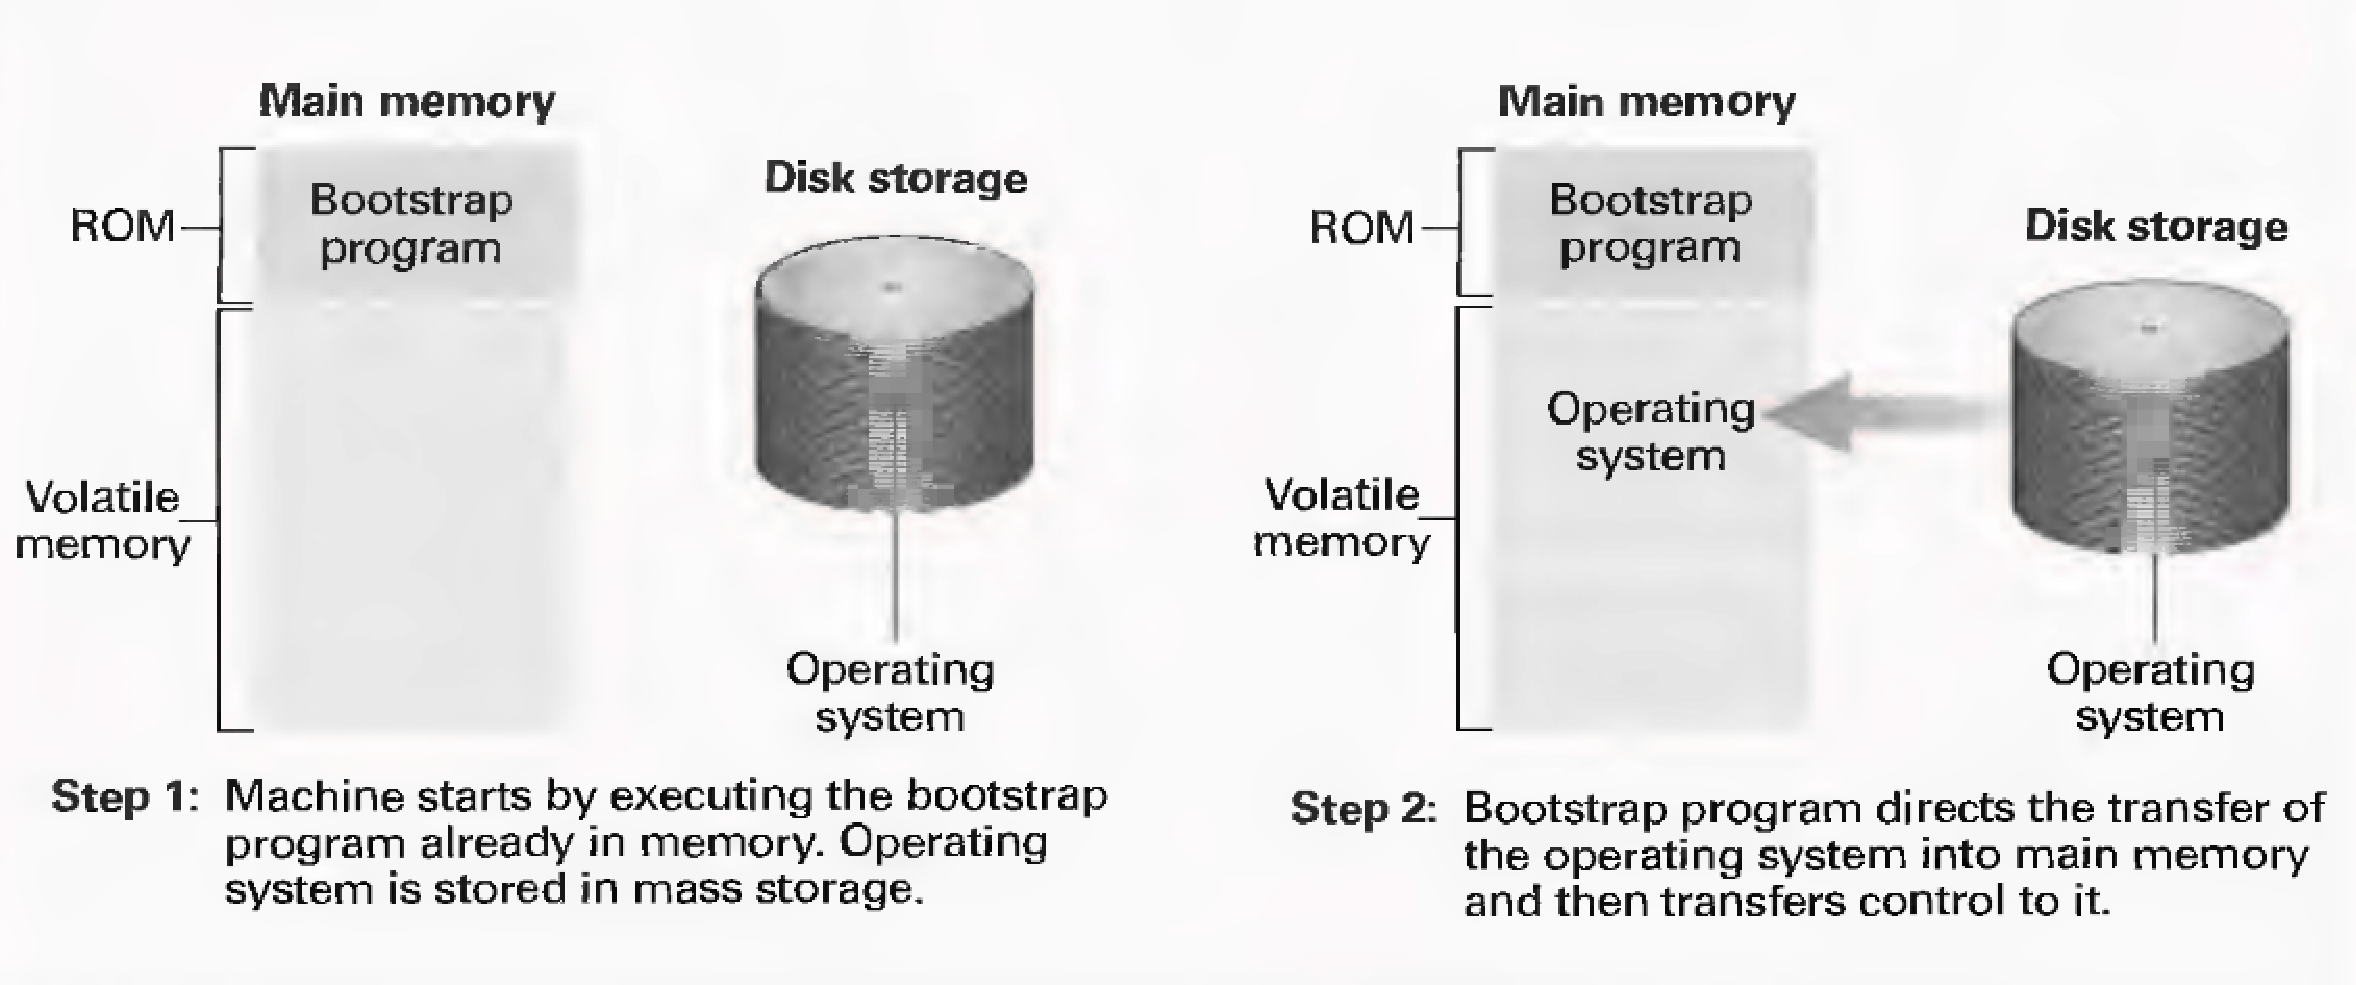
\includegraphics{ch4/fig35.pdf}}
  \caption{Quá trình khởi động}
  \label{fig:fig3.5}
\end{figure}



Một câu hỏi là tại sao không cung cấp đủ ROM để lưu trữ toàn bộ hệ điều hành để tránh phải
nạp từ bộ nhớ thứ cấp. Câu trả lời là do công nghệ hiện tại chưa cho phép dành hẳn một
vùng nhớ lớn của bộ nhớ chính làm vùng lưu trữ bền vững. Tuy nhiên, với sự phát triển
nhanh chóng của công nghệ bộ nhớ, quá trình khởi động mất nhiều bước như thế sẽ sớm trở
nên lạc hâu, và thay vào đó là cách tiếp cận cho phép các phần mềm được lưu trữ lâu bền
trong bộ nhớ.

\subsection*{Câu hỏi \& Bài tập}
\begin{enumerate}
\item Liệt kê các thành phần của một hệ điều hành điển hình và tóm tắt vai trò của mỗi
  thành phần trong một câu.

\item Chỉ ra sự khác nhau giữa phần mềm ứng dụng và phần mềm công cụ.

\item Bộ nhớ ảo là gì?

\item Tóm tắt quá trình khởi động máy.
\end{enumerate}

\section{Điều phối các hoạt động của máy}

Trong phần này ta xem xét cách một hệ điều hành điều phối việc thực hiện phần mềm ứng
dụng, phần mềm công cụ, và bản thân các đơn vị bên trong hệ điều hành. Ta bắt đầu với khái
niệm tiến trình.

\subsection*{Khái niệm tiến trình}
Một trong những khái niệm cơ bản nhất của hệ điều hành hiện đại là phân biệt giữa một
chương trình và hoạt động thực hiện chương trình. Chương trình là một tập tĩnh các chỉ
thị, trong khi đó hoạt động thực hiện chương trình là động, và thay đổi theo thời gian khi
chương trình chạy. Hoạt động này được gọi là \textbf{tiến trình}. Gắn với một tiến trình
là trạng thái hiện hành của hoạt động, được gọi là \textbf{trạng thái của tiến
  trình}. Trạng thái này bao gồm vị trí hiện tại của chương trình đang thực hiện (giá trị
của bộ đếm chương trình) cũng như các giá trị của các thanh ghi và các ô nhớ gắn với
nó. Nói nôm na, trạng thái tiến trình là một ảnh chụp nhanh (snapshot) của máy tại một
thời điểm cụ thể. Những thời điểm khác nhau trong lúc thực hiện chương trình (tại các thời
điểm khác nhau trong một tiến trình) ta quan sát được các ảnh chụp khác nhau (trạng thái
khác nhau của tiến trình).


Trong một hệ thống chia sẻ thời gian thực, thường có nhiều tiến trình tranh chấp tài
nguyên của máy. Nhiệm vụ của hệ điều hành là phải quản lý các tiến trình này sao cho mỗi
tiến trình có tài nguyên (thiết bị ngoại vi, không gian trong bộ nhớ chính, truy cập các
file, và truy cập vào CPU) nó cần, sao cho các tiến trình độc lập không gây trở ngại lẫn
nhau, và sao cho các tiến trình có thể trao đổi thông tin nếu cần.

\subsection*{Quản lý tiến trình}

Các nhiệm vụ liên quan đến việc điều phối tiến trình được thực hiện bởi bộ lập lịch và bộ
điều phối trong nhân của hệ điều hành. Bộ lập lịch duy trì thông tin về tiến trình có mặt
trong hệ thống, đưa các tiến trình mới vào hàng đợi, loại bỏ các tiến trình đã hoàn thành
ra khỏi hệ thống. Bởi vậy, khi người dùng yêu cầu thực hiện một ứng dụng, chính bộ lập
lịch thêm việc thực hiện ứng dụng vào danh sách các tiến trình hiện thời.

Để lưu vết mọi tiến trình, bộ lập lịch duy trì một khối thông tin trong bộ nhớ chính gọi
là \textbf{bảng các tiến trình}. Mỗi khi có yêu cầu thực hiện một chương trình, bộ lập
lịch thêm một mục mới vào trong bảng tiến trình cho tiến trình này. Mục này chứa các thông
tin như vùng bộ nhớ được gán cho tiến trình (lấy từ chương trình quản lý bộ nhớ), độ ưu
tiên của các tiến trình, và trạng thái tiến trình sẵn sàng hay đang đợi. Một tiến trình là
\textbf{sẵn sàng} nếu nó ở trạng thái có thể tiếp tục chạy; nó là \textbf{đợi} nếu hiện
tại nó đang phải đợi cho đến khi một vài sự kiện nào đó bên ngoài xuất hiện, như việc truy
cập đĩa đã hoàn thành, nhấn một phím trên bàn phím, hoặc một thông điệp đến từ tiến trình
khác.



Bộ điều phối tiến trình là thành phần của nhân hệ điều hành chịu trách nhiệm đảm bảo tiến
trình được lập lịch thực sự được thực hiện. Trong hệ thống chia sẻ thời gian thực nhiệm vụ
này được kèm với việc \textbf{chia sẻ thời gian}; có nghĩa rằng, chia thời gian thành
những khoảng ngắn, mỗi khoảng gọi là \textbf{time slide} (thông thường khoảng $50$ mili
giây), và chuyển đổi sự chú ý của CPU tới mỗi tiến trình cho phép mỗi tiến trình thực hiện
trong một time slide (Hình \ref{fig:fig3.6}). Thủ tục chuyển từ tiến trình này sang tiến
trình khác gọi là \textbf{chuyển đổi tiến trình} (process switch) hay \textbf{chuyển ngữ
  cảnh} (context switch).

\begin{figure}[bt]
  \centering \scalebox{0.35}{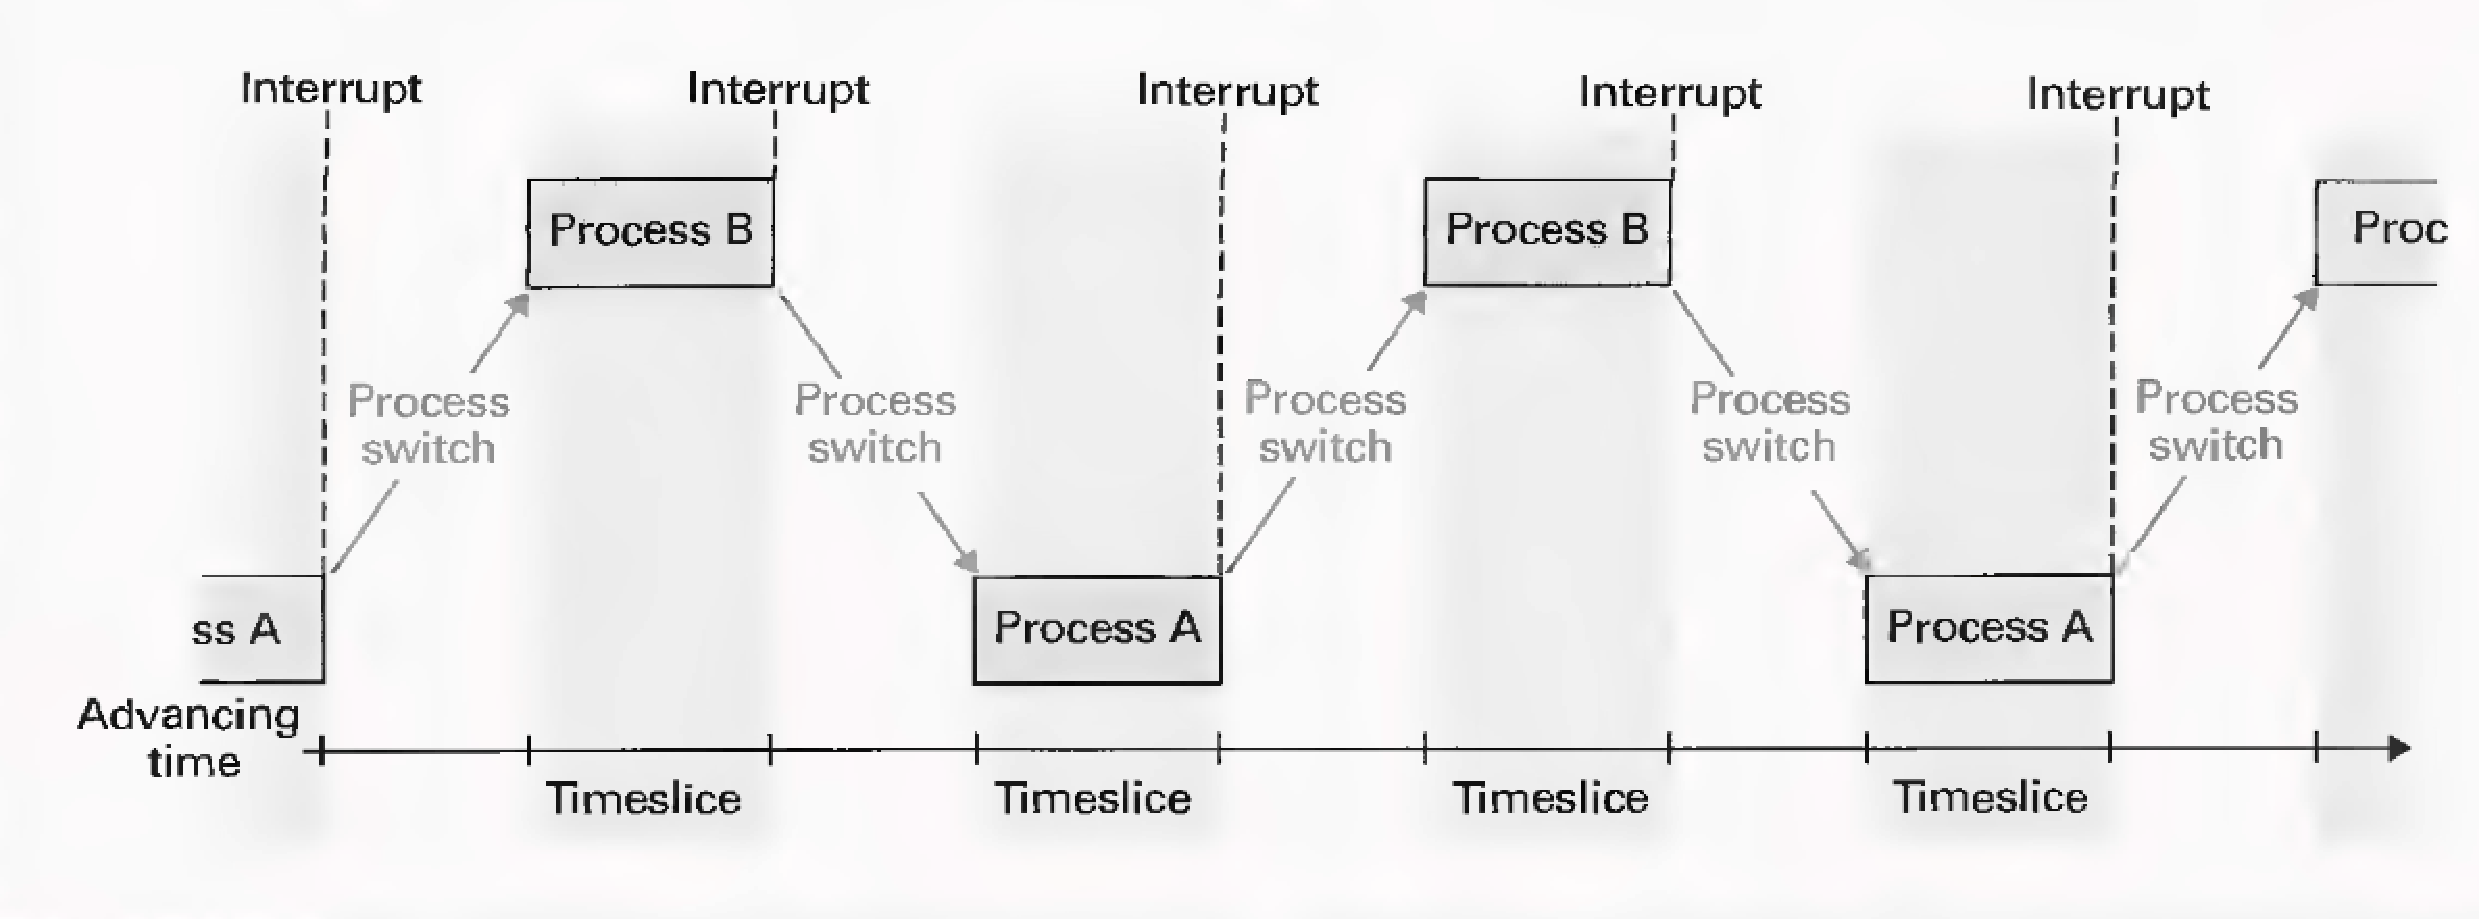
\includegraphics{ch4/fig36.pdf}}
  \caption{Chia sẻ thời gian thực giữa tiến trình $A$ và tiến trình $B$}
  \label{fig:fig3.6}
\end{figure}


Mỗi khi bộ điều phối tiến trình trao time slide cho một tiến trình, nó khởi tạo một mạch
thời gian. Mạch này sẽ sinh ra một tín hiệu gọi là \textbf{ngắt} (interrupt) mỗi khi kết
thúc một time slide. CPU phản hồi lại tín hiệu ngắt này giống như bạn phản ứng khi bị dừng
một công việc. Bạn dừng việc bạn đang làm, ghi nhận lại chỗ công việc bị dừng (để bạn có
thể tiếp tục làm sau), và chuyển sự quan tâm đến đối tượng đòi bạn phải tạm dừng công
việc. Khi CPU nhận một tín hiệu ngắt, nó hoàn thành chu kỳ máy hiện thời của nó, ghi lại
vị trí hiện thời của tiến trình và bắt đầu thực hiện một chương trình, được gọi là
\textbf{trình xử lý ngắt}. Chương trình này được lưu giữ ở một vị trí được xác định trước
trong bộ nhớ chính. Trình xử lý ngắt này là một phần của bộ điều phối, và nó chỉ ra cách
bộ điều phối phải trả lời tín hiệu ngắt.

Bởi vậy, ảnh hưởng của tín hiệu ngắt là để chiếm quyền ưu tiên của tiến trình hiện thời và
chuyển quyền điều khiển lại cho bộ điều phối. Đầu tiên, bộ điều phối cho phép bộ lập lịch
cập nhật bảng các tiến trình (ví dụ, độ ưu tiên của tiến trình vừa hoàn thành time slide
phải thấp hơn độ ưu tiên của các tiến trình khác vừa được đưa vào). Sau đó, bộ điều phối
lựa chọn tiến trình đang sẵn sàng và có độ ưu tiên cao nhất trong bảng các tiến trình,
khởi động lại mạch thời gian, và cho phép tiến trình vừa được lựa chọn bắt đầu time slide
của nó.

Điểm hết sức quan trọng quyết định sự thành công của hệ thống chia sẻ thời gian thực là
khả năng dừng một tiến trình, và sau đó cho phép nó chạy lại. Nếu bạn bị ngắt trong khi
đang đọc sách, khả năng để bạn đọc tiếp sau đó phụ thuộc vào khả năng nhớ vị trí trong
sách cũng như thông tin bạn đã tích luỹ được tính đến thời điểm đó. Nói ngắn gọn, bạn phải
có thể tái tạo lại được môi trường trước thời điểm bị ngắt.

Trong trường hợp của tiến trình, môi trường phải được tái tạo lại là trạng thái của tiến
trình. Nhắc lại rằng trạng thái này bao gồm giá trị của bộ đếm chương trình cũng như nội
dung của các thanh ghi và các ô nhớ thích hợp. Các CPU được thiết kế cho hệ thống chia sẻ
thời gian thực có khả năng kết hợp nhiệm vụ lưu giữ các thông tin này như một phần của
việc phản hồi lại của CPU với tín hiệu ngắt. Các CPU này cũng có các lệnh máy để nạp lại
trạng thái được lưu trữ trước đó. Các đặc điểm này đơn giản hoá nhiệm vụ của bộ điều phối
khi thực hiện chuyển đổi tiến trình và cũng là một ví dụ cho thấy việc thiết kế các CPU
hiện đại bị ảnh hưởng bởi nhu cầu của các hệ điều hành thế nào.

Cuối cùng, ta cũng để ý rằng việc chia sẻ thời gian thực làm tăng hiệu quả của hệ thống về
mặt tổng thể. Điều này đôi khi ngược lại với trực giác của ta vì việc chuyển đổi giữa các
tiến trình yêu cầu bởi hệ thời gian thực làm tốn thời gian của CPU. Tuy nhiên, nếu không
chia sẻ thời gian thực, mỗi tiến trình sẽ phải hoàn thành việc thực hiện trước khi tiến
trình tiếp theo bắt đầu, có nghĩa rằng thời gian tiến trình đợi thiết bị ngoại vi hoàn
thành hoặc đợi yêu cầu từ người sử dụng là bị lãng phí. Còn nếu chia sẻ thời gian thực sẽ
cho phép chuyển CPU đang đợi cho tiến trình khác. Ví dụ, nếu một tiến trình thực hiện một
yêu cầu vào/ra, ví dụ yêu cầu lấy dữ liệu từ đĩa, bộ lập lịch sẽ cập nhật bảng tiến trình
để phản ánh rằng tiến trình này đang đợi một sự kiện bên ngoài. Vậy, bộ điều phối sẽ cắt
time slide của tiến trình này. Sau đó (có thể đến vài nghìn mili giây), khi yêu cầu vào/ra
được hoàn thành, bộ lập lịch sẽ cập nhật bảng tiến trình để chỉ ra rằng tiến trình là sẵn
sàng, và bởi vậy tiến trình này sẽ một lần nữa cạnh tranh để lấy time slides. Tóm lại, một
tiến trình vẫn có thể được thực hiện trong khi yêu cầu vào/ra đang được thực hiện. Bởi
vậy, các nhiệm vụ sẽ được hoàn thành mất ít thời gian hơn so với thực hiện theo cách tuần
tự.

\subsection*{Câu hỏi \& Bài tập}
\begin{enumerate}
\item Tóm tắt sự khác nhau giữa chương trình và tiến trình.

\item Tóm tắt các bước được thực hiện bởi CPU khi một ngắt xuất hiện.

\item Trong hệ thống chia sẻ thời gian, làm thế nào các tiến trình có
  độ ưu tiên cao được phép chạy nhanh hơn so với các tiến trình khác?

\item Nếu mỗi time slide trong hệ thống chia sẻ thời gian là $50$
  milli giây và mỗi việc chuyển đổi ngữ cảnh yêu cầu ít nhất một micro
  giây, có bao nhiêu tiến trình có thể được phục vụ trong một giây?
\label{ex:3.3.4}

\item Nếu mỗi tiến trình sử dụng đầy đủ time slide của nó theo máy ở
  Bài tập \ref{ex:3.3.4}, khoảng thời gian nào của máy thực sự dành
  cho việc thực hiện tiến trình? khoảng thời gian của máy thực sự dành
  cho thực hiện tiến trình là bao nhiêu nếu mỗi tiến trình thực hiện
  một yêu cầu vào/ra chỉ sau một micro giây time slide của nó?
\end{enumerate}







%%% Local Variables: 
%%% mode: latex
%%% TeX-master: "../tindaicuong"
%%% End: 


\section{An ninh của máy tính}

Bởi vì các hệ điều hành giám sát các hoạt động của máy tính, nên nó cũng đóng vai trò
chính trong việc đảm bảo an ninh. Theo nghĩa rộng, nó có thể ở nhiều dạng, một trong số
chúng là độ tin cậy. Nếu sai sót trong trình quản lý file gây ra mất dữ liệu của file, vậy
file không an toàn. Nếu chương trình điều phối gây ra đổ vỡ hệ thống, làm mất dữ liệu ta
mất cả giờ để đánh, vậy công việc của ta không an toàn. Bởi vậy, an ninh của một hệ
thống tính toán đòi hỏi hệ điều hành phải được thiết kế tốt và đáng tin cậy.

Việc phát triển các phần mềm đáng tin cậy không phải là vấn đề nghiên cứu của hệ điều
hành. Nó thuộc phạm vi của Công nghệ phần mềm, ta sẽ xem xét sau trong
Chương~\ref{}. Trong phần này, ta chỉ quan tâm đế các vấn đề an ninh liên quan riêng đến
hệ điều hành.

\subsection*{Tấn công từ bên ngoài}
Một trong những nhiệm vụ quan trọng của hệ điều hành là bảo vệ tài nguyên của máy tính
tránh khỏi các truy cập bất hợp lệ. Trong trường hợp hệ thống có nhiều người sử dụng, việc
bảo vệ này dựa trên ``tài khoản'' (account)--một tài khoản được quản lý trong trong hệ
điều hành như một mục gồm tên người dùng, mật khẩu và quyền truy cập gắn với người
dùng. Hệ điều hành dùng các thông tin này trong mỗi lần đăng nhập (login) để điều khiển
việc truy cập vào hệ thống.

Các tài khoản được tạo bởi một người gọi là \textbf{super user} hay \textbf{người quản
  trị} (administrator). Người này có quyền cao nhất trong hệ thống, và cũng phải đăng nhập
vào hệ thống để xác thực anh/chị ta là người quản trị (thường bởi tên và mật khẩu). Khi đã
đăng nhập, người quản trị có thể làm nhiều thay đổi bên trong hệ thống như: thay đổi gói
phần mềm, gán quyền cho người dùng, thực hiện các hoạt động bảo trì hệ thống,...

Dùng ``quyền rất cao'' này, người quản trị phải điều khiển hoạt động trong hệ thống để
kiểm tra các hành vi phá hoại hệ thống, do vô tình hay cố ý. Cũng có nhiều phần mềm công
cụ trợ giúp người quản trị, được gọi là \textbf{phần mềm kiểm tra} (auditing software). Nó
ghi lại và phân tích các hoạt động xảy ra bên trong hệ thống. Ví dụ, phần mềm kiểm tra có
thể cho biết những lần đăng nhập sai mật khẩu. Phần mềm kiểm tra cũng phát hiện các hoạt
động của một tài khoản người dùng không phù hợp với các hành vi của anh ta trong quá khứ,
để từ đó chỉ ra những người dùng không có thẩm quyền đã giành được quyền truy cập vào tài
khoản này. (ví dụ, với một người dùng bình thường chỉ dùng gói phần mềm xử lý văn bản và
bảng tính, bây giờ lại dùng các ứng dụng phần mềm kỹ thuật cao hoặc thực hiện các gói công
cụ không hợp lệ với quyền của anh ta.)

Phần mềm kiểm tra cũng được thiết kế để phát hiện các \textbf{phần mềm sniffing}, là phần
mềm khi được phép chạy trên hệ thống sẽ tìm cách ghi lại các hoạt động và sau đó thông báo
lại cho kẻ thâm nhập (intruder). Một ví dụ tuy cũ nhưng được biết rộng rãi là một chương
trình một phỏng thủ tục đăng nhập của hệ điều hành. Các chương trình như thế này có thể
làm cho người dùng khác nhầm tưởng họ đang giao tiếp với hệ điều hành, và cung cấp tên và
mật khẩu cho kẻ mạo danh.

Với mọi sự phức tạp về mặt kỹ thuật được gắn với máy tính, thật đáng ngạc nhiên là rào cản
chính của an ninh của máy tính là do sự thiếu thận trọng của người dùng. Họ chọn các mật
khẩu rất dễ đoán (như tên và ngày sinh), họ chia sẻ mật khẩu của họ với bạn bè, họ không
thay đổi mật khẩu thường xuyên, họ đưa các thiết bị lưu trữ khối off-line của mình đến chỗ
hỏng hóc khi họ chuyển các thiết bị này giữa các máy, họ cài đặt các phần mềm có thể gây
mất an toàn vào hệ thống. Để giải quyết những vấn đề này, hầu hết các hệ thống máy tính
lớn đều bắt ép người dùng tuân theo một số yêu cầu về an toàn để nâng cao ý thức trách
nhiệm của họ.

\subsection*{Tấn công từ bên trong}
Khi một kẻ thâm nhập (có thể là người dùng hợp lệ nhưng có ý đồ xấu) tấn công vào hệ
thống, chúng thường tìm cách thăm dò, tìm các thông tin quan tâm, hoặc cài đặt vào hệ
thống các phần mềm phá hoại. Điều này rất đơn giản nếu kẻ rình mò có thể truy cập hệ thống
bằng tài khoản của người quản trị. Đây chính là lý do tại sao mà mật khẩu của người quản
trị phải được bảo vệ một cách nghiêm ngặt. Tuy nhiên, nếu truy cập được vào tài khoản
người dùng thông thường, kẻ thâm nhập phải tìm cách làm đánh lừa hệ điều hành để truy cập
vào các vùng bị cấm. Ví dụ, kẻ truy cập có thể đánh lừa trình quản lý bộ nhớ cho phép một
tiến trình truy cập ra ngoài vùng nhớ dành cho nó, hoặc kẻ truy cập có thể cố gắng đánh
lừa trình quản lý file để lấy các file mà nó không có quyền truy cập.


Các CPU hiện đại được thiết kế có thêm các đặc tính nhằm ngăn chặn những vấn đề này. Ví
dụ, có thể xét nhu cầu hạn chế một tiến trình chỉ được truy cập vào vùng bộ nhớ mà trình
quản lý bộ nhớ gán cho nó; nếu không hạn chế, một tiến trình có thể xoá hệ điều hành trong
bộ nhớ chính và chiếm quyền điều khiển máy tính. Để ngăn chặn vấn đề này, các CPU được
thiết kế cho hệ điều hành đa nhiệm có thể chứa các thanh ghi đặc biệt cho phép hệ điều
hành lưu giữ các giới hạn trên và dưới của vùng nhớ được gán cho tiến trình. Và trong khi
thực hiện xử lý, CPU so sánh mỗi vùng nhớ được tham chiếu đến với các thanh ghi này để đảm
bảo nó nằm trong giới hạn cho phép. Nếu vùng nhớ tham chiếu đến vượt ra ngoài giới hạn
này, CPU tự động chuyển quyền điều khiển tới hệ điều hành (bằng cách thực hiện một dãy các
ngắt) để hệ điều hành có các xử lý phù hợp.

Dù đặc điểm ta mô tả ở trên có vẻ rất tinh tế, nhưng trên thực tế nó vẫn có vấn đề. Nếu
CPU không có thêm một vài đặc tính an toàn nữa, một tiến trình vẫn có thể truy cập vào các
ô nhớ bất hợp lệ bằng cách thay đổi thanh ghi đặc biệt (chứa giới hạn bộ nhớ). Có nghĩa
rằng, một tiến trình có thể truy cập một bộ nhớ bên ngoài đơn thuần bằng cách thay đổi các
giá trị trong thanh ghi chứa giới hạn trên và dưới của bộ nhớ, và do đó nó có thể sử dụng
không gian bộ nhớ thêm mà không cần hệ điều hành cho phép.

Để tránh các hoạt động kiểu này, CPU được thiết kế để có thể thực hiện trong một hoặc hai
\textbf{mức đặc quyền} (privilege level); ta sẽ gọi là ``mode đặc quyền'' và ``mode
không đặc quyền.'' Khi ở trong mode đặc quyền, CPU có thể thực hiện mọi lệnh có trong ngôn
ngữ máy của nó. Tuy nhiên, khi ở trong mode không đặc quyền, các lệnh mà nó có thể thực
hiện sẽ bị giới hạn. Các lệnh chỉ được phép chạy ở mode đặc quyền gọi là \textbf{lệnh đặc
  quyền}. (ví dụ lệnh đặc quyền điển hình là lệnh làm thay đổi nội dung các thanh ghi giới
hạn bộ nhớ và các lệnh làm thay đổi mode đặc quyền của CPU.) Mọi nỗ lực thực hiện một lệnh
đặc quyền khi CPU ở mode không đặc quyền đều gây ra một ngắt. Ngắt này chuyển CPU tới mode
đặc quyền và chuyển quyền điều khiển tới trình xử lý ngắt của hệ điều hành.

Khi máy được bật, CPU ở mode đặc quyền. Bởi vậy, khi kết thúc quá trình khởi động và hệ
điều hành chiếm quyền điều khiển, lúc này mọi lệnh máy đều có thể được hiện. Tuy nhiên,
mỗi khi hệ điều hành cho phép một tiến trình chạy một time slide, nó chuyển CPU tới mode
không đặc quyền bằng cách thực hiện một lệnh ``chuyển mode đặc quyền''. Và từ lúc này, hệ
điều hành sẽ được thông báo nếu tiến trình cố gắng thực hiện lệnh ở mode đặc quyền.

Các lệnh đặc quyền và điều khiển các mức đặc quyền là các công cụ chính sẵn có để các hệ
điều hành quản lý an ninh. Tuy nhiên, việc sử dụng các công cụ này là một công việc hết
sức phức tạp trong thiết kế hệ điều hành. Một lỗi nhỏ trong điều khiển mức đặc quyền có
thể gây ra thảm hoạ do những người lập trình có ý đồ xấu hoặc do các lỗi vô ý gây ra khi
lập trình. Nếu một tiến trình được phép thay đổi thay đổi bộ định thời gian điều khiển
việc chia sẻ thời gian thực của hệ thống có thể cho phép một tiến trình mở rộng time slide
và chiếm quyền điều khiển máy. Nếu một tiến trình được phép truy cập trực tiếp vào thiết
bị ngoại vi, vậy nó có thể đọc các file mà không bị giám sát bởi trình quản lý file. Nếu
một tiến trình được phép truy cập vào các ô nhớ bên ngoài vùng cho phép, nó có thể đọc và
thậm chí thay đổi dữ liệu đang được sử dụng bởi tiến trình khác.
  
\subsection*{Câu hỏi \& Bài tập}
\begin{enumerate}
\item Hãy cho vài ví dụ về việc chọn mật khẩu kém an toàn và giải thích tại sao chúng lại
  kém?

\item Các bộ xử lý của Intel sử dụng bốn mức đặc quyền. Tại sao người thiết kế lại quyết
  định dùng bốn mà không phải là ba hay năm mức?

\item Nếu một tiến trình trong hệ thống chia sẻ thời gian thực có thể truy cập vào vùng
  nhớ không được phép, làm thế nào nó có thể chiếm quyền điều khiển máy?
\end{enumerate}
%%% Local Variables: 
%%% mode: latex
%%% TeX-master: "../tindaicuong"
%%% End: 

\section{Bài tập cuối chương}
  

\begin{multicols}{2}
  \begin{enumerate}
  \item Liệt kê bốn hoạt động của một hệ điều hành điển hình.

  \item Tóm tắt sự khác nhau giữa xử lý theo lô và xử lý tương tác.

  \item Ta đặt (theo thứ tự) ba phần tử $R, S$ và $T$ vào trong một
    hàng đợi. Đầu tiên, ta lấy hai phần tử ra khỏi hàng đợi và đặt
    thêm một phần tử $X$ vào hàng đợi. Sau đó, ta lại lấy tiếp hai
    phần tử ra khỏi hàng đợi, và lại đặt thêm hai phần tử $Y, Z$ (theo
    thứ tự) vào hàng đợi, và sau đó lấy hết các phần tử cho đến khi
    hàng đợi rỗng. Hãy liệt kê các phần tử trong hàng đợi theo thứ tự
    mà chúng bị lấy ra.

  \item Chỉ ra sự khác biệt giữa xử lý tương tác và xử lý thời gian
    thực.

  \item Hệ điều hành đa nhiệm là gì?

  \item Giả sử bạn có một máy PC, hãy chỉ ra một vài tình huống bạn
    thấy rõ lợi thế của khả năng đa nhiệm của nó.

  \item Hãy chỉ ra hai phần mềm ứng dụng và hai phần mềm công cụ mà
    bạn quen thuộc.

  \item Cấu trúc thư mục được mô tả bởi đường dẫn X/Y/Z là gì?

  \item Bảng mô tả tiến trình chứa những thông tin gì?

  \item Chỉ ra sự khác nhau giữa tiến trình sẵn sàng và tiến trình
    đang đợi.

  \item Nêu sự khác nhau giữa bộ nhớ ảo và bộ nhớ chính.

  \item Giả sử máy tính của bạn có $512$MB (MiB) bộ nhớ chính, và một
    hệ điều hành cần tạo một bộ nhớ ảo gấp hai lần kích thước bộ nhớ
    chính với kích thước các trang được dùng là $2$KB (KiB). Có bao
    nhiêu trang có thể được yêu cầu.

  \item Vấn đề phức tạp gì xảy ra trong hệ thống chia sẻ thời gian
    thực nếu hai tiến trình yêu cầu truy cập vào cùng một file tại
    cùng một thời điểm? Có trường hợp nào mà trình quản lý file nên
    cho phép các yêu cầu kiểu này? Có trường hợp nào mà trình quản lý
    file nên cấm các yêu cầu kiểu này?

  \item Định nghĩa cân bằng tải và tỷ xích (scaling) trong ngữ cảnh của kiến
    trúc đa bộ xử lý.

  \item Tóm tắt quá trình khởi động máy.

  \item Giả sử bạn có một máy PC, hãy ghi lại dãy các hoạt động mà bạn
    quan sát được khi bật máy. Sau đó hãy xác định các thông điệp được
    hiện lên màn hình máy tính trước khi quá tình khởi động thực sự
    bắt đầu. Phần mềm gì viết các thông điệp này?

  \item Giả sử rằng hệ điều hành chia sẻ thời gian thực cấp phát các time slide~$20$mili
    giây và máy thực hiện trung bình $5$ lệnh trong một micro giây. Vậy máy có thể thực
    hiện bao nhiêu lệnh trong một time slide?

  \item Nếu một người đánh được $60$ từ trong một phút (một từ được xem là gồm $5$ ký tự),
    vậy mỗi ký tự người đó đánh mất bao lâu?  nếu người đó dùng một hệ điều hành chia sẻ
    thời gian thực cấp phát time slide theo đơn vị~$20$ mili giây và chúng ta bỏ qua việc
    chuyển đổi giữa các tiến trình, vậy có bao nhiêu time-slide có thể được cấp phát giữa
    lúc hai ký tự được đánh?


  \item Giả sử một hệ điều hành chia sẻ thời gian thực chia time slide là~$50$ milli
    giây. Nếu bình thường đầu đọc/ghi đĩa mất $8$ milli giây để chuyển tới track mong muốn
    và mất thêm $17$ mili giây để tới dữ liệu mong muốn, vậy một chương trình mất bao
    nhiêu time slide để đợi thao tác đọc đĩa hoàn thành? Nếu máy có khả năng thực hiện
    mười lệnh mỗi micro giây, bao nhiêu lệnh có thể thực hiện trong khi đợi chu kỳ này?
    (Đây là lý do tại sao khi một tiến trình thực hiện một thao tác với thiết bị ngoại vi,
    hệ thống chia sẻ thời gian thực kết thúc time slide của tiến trình này và cho phép
    tiến trình khác chạy trong khi tiến trình ban đầu đợi phục vụ của thiết bị ngoại vi.)


  \item Liệt kê năm nguồn tài nguyên mà hệ điều hành đa nhiệm phải
    điều phối việc truy cập.


  \item Một tiến trình được gọi là I/O-bound nếu nó yêu cầu nhiều phép
    toán vào/ra, còn một tiến trình được gọi là compute-bound nếu hầu
    hết thời gian thực hiện nó dành cho việc tính toán. Giả sử có hai
    tiến trình, một là I/O-bound và một là compute-bound, đang cùng
    đợi một time-slide, vậy ta nên ưu tiên tiến trình nào? Tại sao?

  \item Trong một hệ thống chia sẻ thời gian thì hiệu suất chạy hai
    tiến trình I/O bound tốt hơn hay chạy một tiến trình I/O bound và
    một compute-bound tốt hơn? Tại sao?

  \item Viết các chỉ thị mà bộ điều phối của hệ điều hành phải làm khi
    một tiến trình hết time slide.

  \item Trạng thái của tiến trình gồm những thành phần gì?

  \item Chỉ ra một tình huống mà một tiến trình trong hệ thống chia sẻ
    thời gian thực không dùng hết time slide được cấp cho nó.

  \item Liệt kê theo thứ tự thời gian các sự kiện xuất hiện khi một
    tiến trình bị ngắt.

  \item Trả lời các câu hỏi sau đây theo hệ điều hành bạn đang dùng:
    \begin{enumerate}[a.]
    \item Làm thế nào để yêu cầu hệ điều hành copy một file từ vị
      trí này tới vị trí khác?

    \item Làm thế nào để xem các thư mục trên đĩa?

    \item Làm thế nào để yêu cầu hệ điều hành thực hiện một chương trình?
    \end{enumerate}

  \item Trả lời các câu hỏi sau đây theo hệ điều hành bạn đang dùng:
    \begin{enumerate}[a.]
    \item Làm thế nào hệ điều hành hạn chế truy cập chỉ cho những
      người được phép?

    \item Làm thế nào để yêu cầu hệ điều hành chỉ ra các tiến trình
      hiện đang có trong bảng tiến trình?

    \item Làm thế nào để bảo hệ điều hành rằng bạn không muốn người
      dùng khác truy cập vào file của bạn?
    \end{enumerate}

  \item Làm thế nào một hệ điều hành giữ không cho một tiến trình truy
    cập vào không gian bộ nhớ của tiến trình khác?

  \item Giả sử một mật khẩu bao gồm một xâu chín ký tự trong bảng chữ
    cái Tiếng Anh ($26$ ký tự). Nếu mỗi mật khẩu có thể được kiểm tra
    trong một milli giây, vậy mất bao lâu có thể kiểm tra mọi mật khẩu
    có thể?

  \item Tại sao các CPU thiết kế cho hệ điều hành đa nhiệm lại cần
    phân chia các thao tác theo các mức đặc quyền khác nhau?

  \item Hãy chỉ ra hai hoạt động yêu cầu các lệnh đặc quyền?

  \item Hãy chỉ ra ba cách mà một tiến trình có thể gây mất an toàn
    cho hệ thống máy tính nếu hệ điều hành không ngăn chặn.
  \end{enumerate}
\end{multicols}


%%% Local Variables: 
%%% mode: latex
%%% TeX-master: "../tindaicuong"
%%% End: 
   
%%% Local Variables: 
%%% mode: latex
%%% TeX-master: "../tindaicuong"
%%% End: 
